\chapter{Porównanie metod detekcji - eksperymenty}

Podczas eksperymentowania z~różnymi algorytmami i~metodami detekcji,
rozpoznawania obiektów, oraz obróbki obrazów powstało wiele implementacji
najbardziej obiecujących rozwiązań. Wiele z~nich od razu nie dawało 
zadowalających rezultatów, inne były zupełnie niezwiązane z~zagadnieniem,
a~jeszcze inne zostały popełnione aby zachować pozory użyteczności 
i~przydatności rozwiązania omawianego problemu w~codziennym życiu.

W~tym rozdziale przedstawione i~pokrótce opisane zostały kroki podjęte
w~celu znalezienia najbardziej optymalnego rozwiązania postawionego 
problemu. 
W~pierwszej kolejności przedstawiono kilka ślepych uliczek, które 
nie zostały uwzględnione w~rozwiązaniu końcowym. W~kolejnym podrozdziale
pokazano szereg prób weryfikacji skuteczności i~optymalizacji 
poszczególnych kroków ostatecznego algorytmu. W~podsumowaniu uwzględniono
częściowo przypadkowo zidentyfikowane właściwości zastosowanych
narzędzi oraz implementacji, a także wpływ tychże odkryć na ostateczny
kształt finalnego rozwiązania.

\section{Eksperymenty nieudane}

W~tym podrozdziale przedstawione zostały próby, których wykonanie
skutkowało jedynie zwiększeniem świadomości na temat zagadnienia.
Główną przyczyną niewykorzystania zamieszczonych tutaj pomysłów
była niepewność co do skuteczności, bądź wydajności rozwiązania końcowego
które miało by być na nich oparte.

Pozostałe przyczyny to m.in. niedostosowanie rozważanego rozwiązania
do omawianego problemu. Ostatecznie zbyt duży nakład pracy, która
byłaby wymagana do dostosowania potencjalnej implementacji do
stawianych wymagań, np.: optymalizacja wysokiej złożoności obliczeniowej
lub przepisanie złożonego algorytmu na język JAVA (środowisko android)
jeżeli istniały tylko implementacje w~innych językach.

\subsection{Biblioteka OpenTLD}

Pierwszym przeciwwskazaniem do wykorzystania biblioteki OpenTLD 
był brak implementacji w~języku JAVA. Algorytm wydawał się na tyle
skomplikowany, że samo jego przeportowanie ze środowiska MatLab,
czy nawet implementacji w~C++ mogło by stanowić zakres pracy
mniejszego kalibru (inżynierskiej) lub projektu zespołowego.
Pomimo to podjęto próbę kontrolną mającą na celu sprawdzenie
skuteczności i~przydatności wspomnianego rozwiązania we wstępnej 
segmentacji - pierwszy krok proponowanej kaskady.

\begin{figure}[h!]
    \caption{Niestabilność i niedokładność rezultatów uzyskanych przy
    użyciu biblioteki OpenTLD}
    \centering
    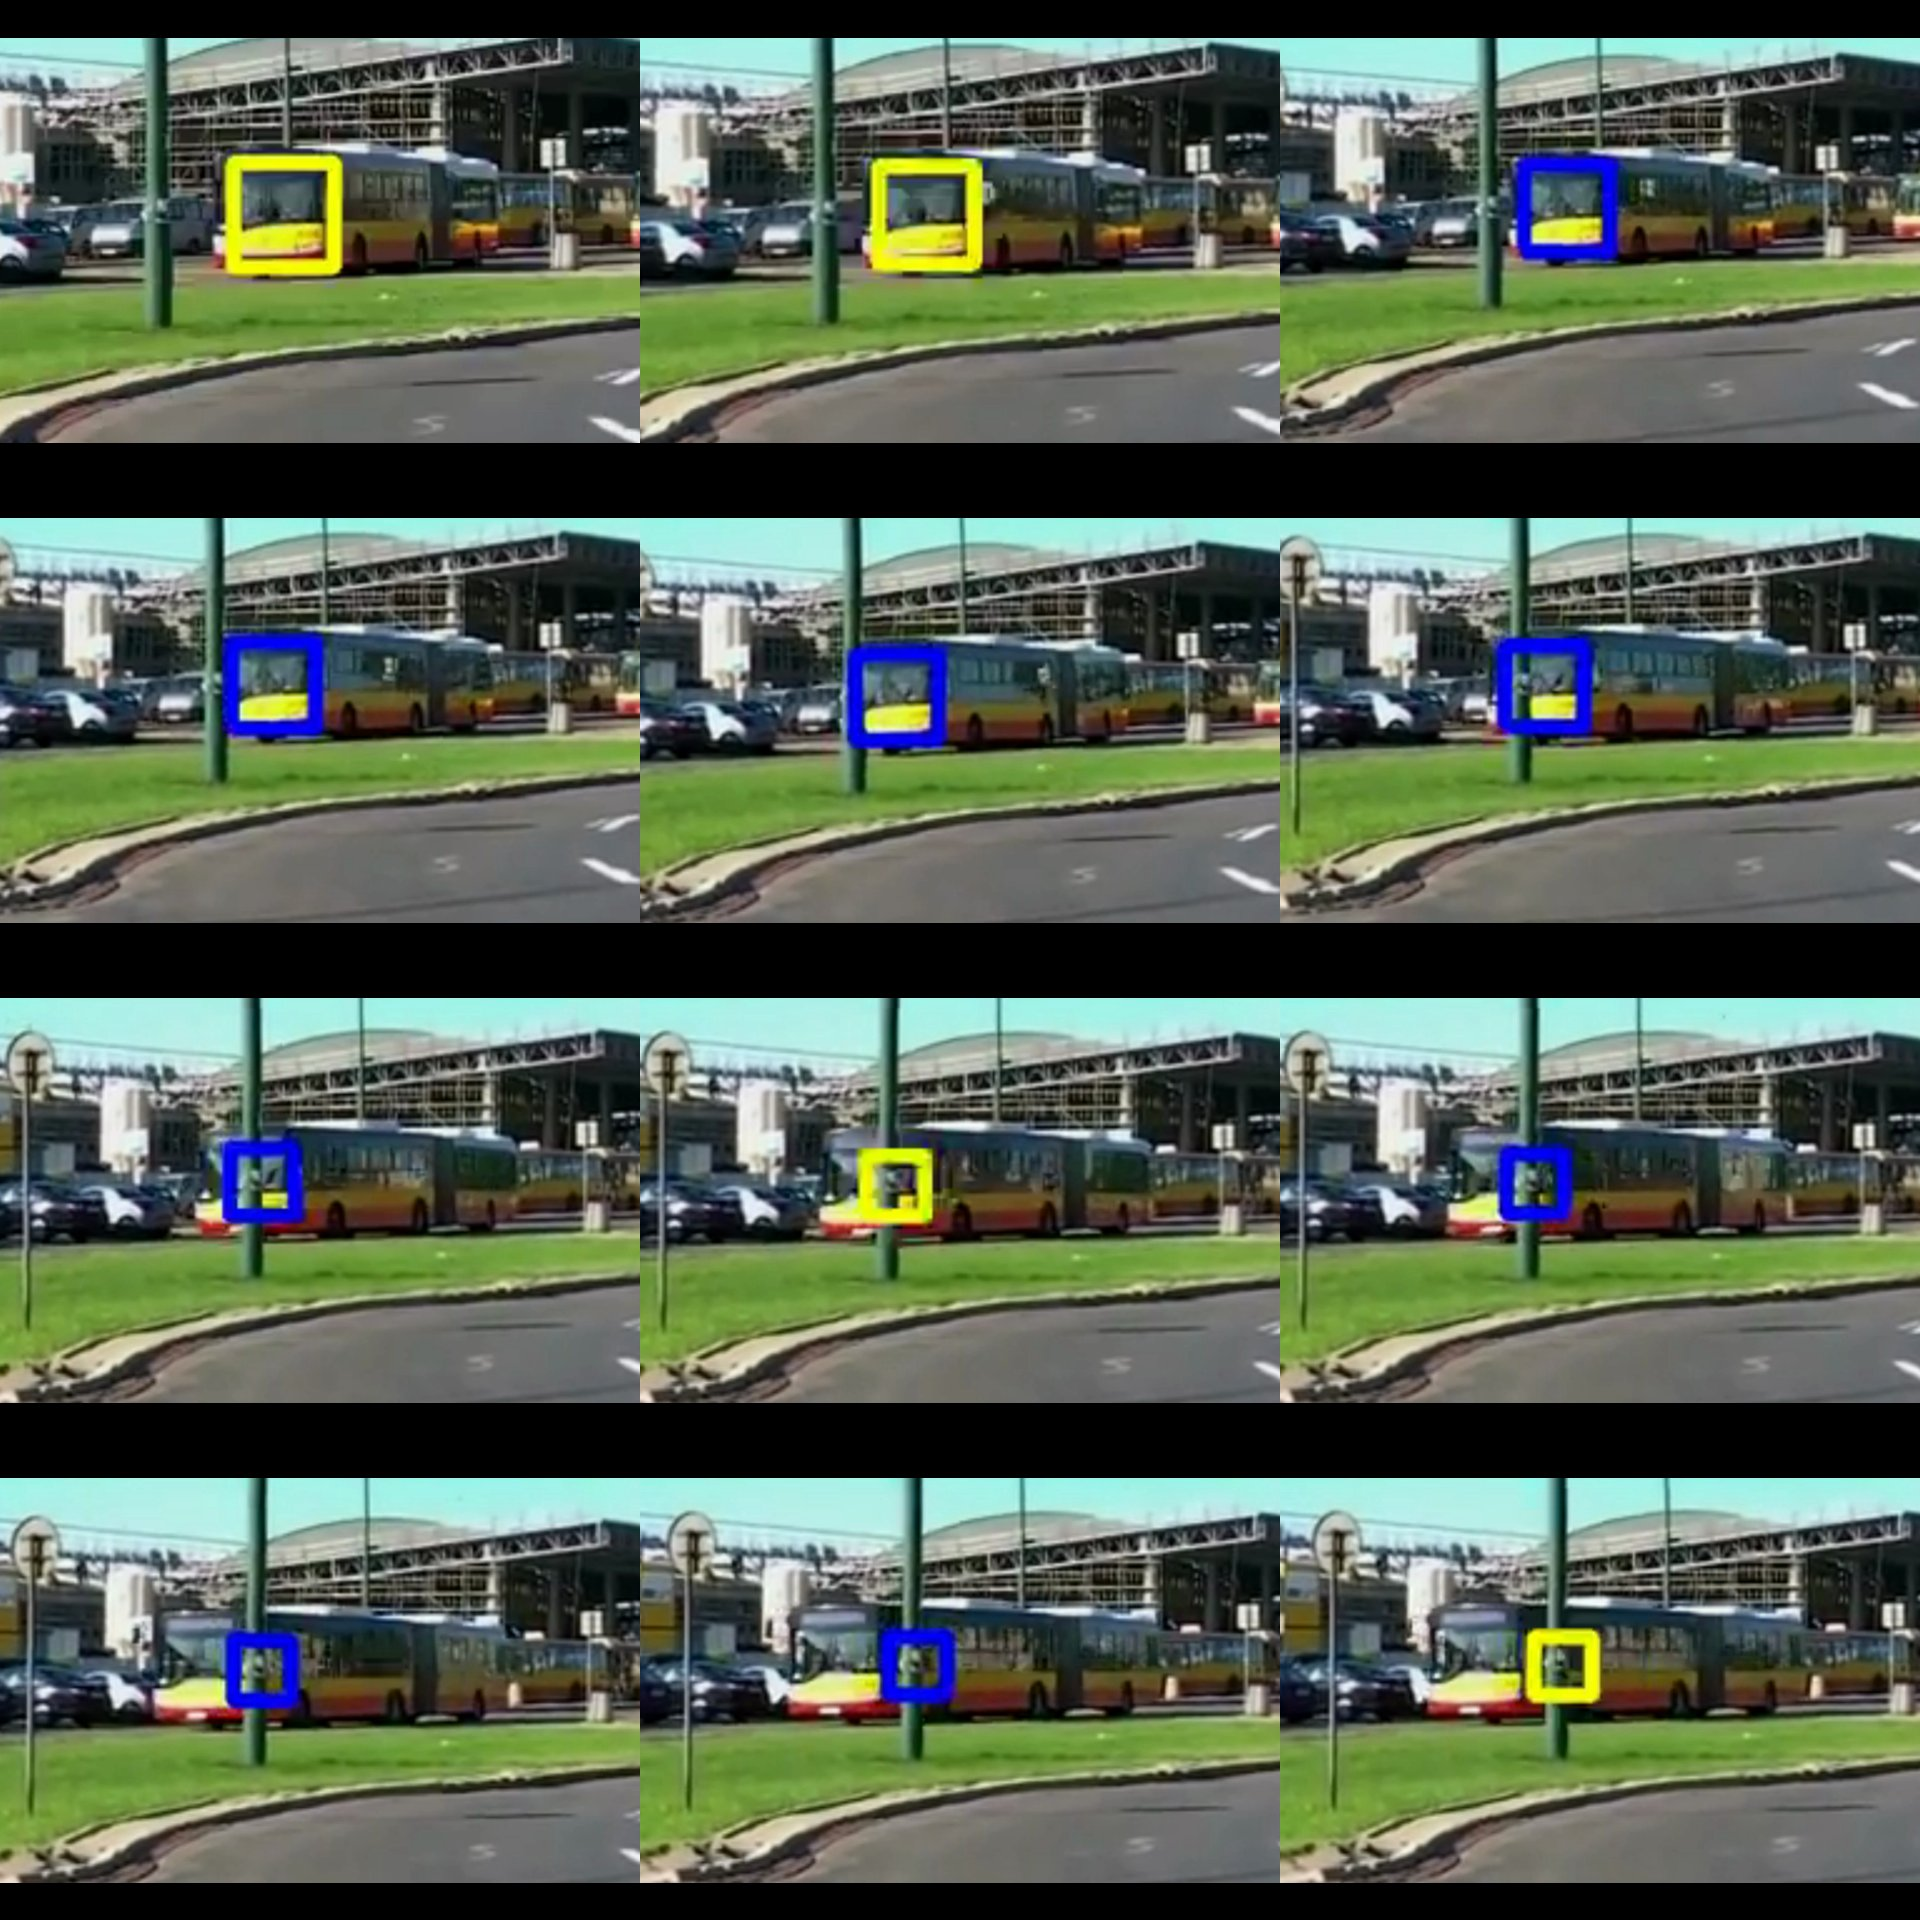
\includegraphics[width=0.9\textwidth]{img/exp_open_tld_fail}
\end{figure}

Skuteczność wykrywania frontów autobusów (potwierdzona 
niestety jedynie organoleptycznie) była więcej niż zadowalająca.
Liczba trafień uzyskanych z~pojedynczego wstępnego zaznaczenia frontu
była niemal stu procentowa. Niestety dokładność wykrytych obiektów
była poniżej oczekiwanej. Standardowo zdarzały się problemy
obciętych numerów - zbyt mały czworokąt okalający. Dodatkowo
brak możliwości ingerencji w~proces uczenia detektora oraz jego
duże tendencje do ,,pływania'' skutkowały nieraz wynikami pozytywnymi
typu: lewy dolny róg frontu do 1/2 wysokości i~szerokości. 

Na rysunku powyżej można zaobserwować zupełne zgubienie obiektu 
śledzonego - 
front autobusu - na rzecz słupa. Wynik tego eksperymentu oraz
zaobserwowany spadek wydajności - ilość obsłużonych klatek na sekundę - 
dla rosnącej liczby zebranych pozytywnych i~negatywnych próbek
(na powyższym rysunku żółte kwadraty oznaczają próbkę, która została
wykorzystana do procesu uczenia detektora) 
wpłynęły na decyzję zaprzestania dalszych testów biblioteki OpenTLD.
Ostatecznie dla jednej sesji,
nagrania długości około 5 minut, wydajność potrafiła spaść z~poziomu
początkowych 20 fps do nawet 2 klatek na sekundę. Poprawa tego stanu 
rzeczy była by co najmniej nie na miejscu. Szczególnie, że Pan 
Zdenek Kalal wydał drugą wersję biblioteki TLD (tym razem już nie 
open), której jednym z~usprawnień był właśnie znaczny wzrost wydajności
\cite{WEB:kalaltld2}.

\subsection{Wykrywanie linii krawężnika zatoki autobusowej}

Rozpoczynając ten podrozdział, trudno nie zacząć go od cytatu:
,,A~teraz coś z~zupełnie innej beczki''. Po podjęciu decyzji o~rezygnacji
z~wykorzystania
biblioteki OpenTLD, w~ramach poszukiwań optymalnego sposobu wstępnej
segmentacji użyty został filtr ,,Canny'' z~pakietu OpenCV. Celem prac
miał być detektor krawędzi, który mógłby zostać użyty do
wykrycia górnej krawędzi frontu autobusu lub zarysu autobusu w~ogóle.
Po wykryciu bliżej niezdefiniowanego zestawu pionowych i~poziomych
krawędzi oraz zastosowaniu co do niego takich samych (bliżej
niezdefiniowanych) ograniczeń geometrycznych, algorytm miałby
stwierdzić, że fragment którego cechy spełniają pewne kryteria jest
właśnie frontem autobusu.

Patrząc na kilka wynikowych obrazów reprezentujących wykryte krawędzie,
okazało się, że najlepiej 
widoczną linią (krawędzią) jest linia wyznaczona przez krawężnik
zatoki autobusowej.

\begin{figure}[h!]
    \caption{Wykrywacz linii krawędzi zatoki autobusowej}
    \centering
    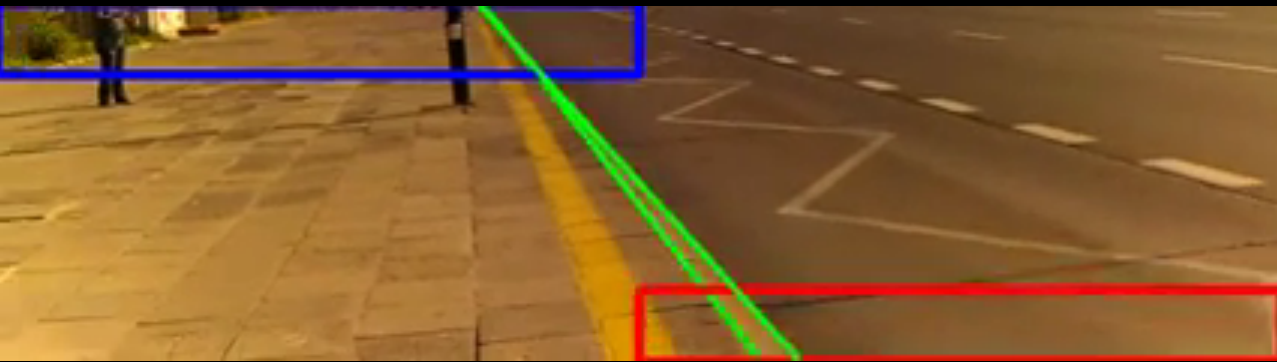
\includegraphics[width=0.9\textwidth]{img/exp_bus_lane_edge_detector}
\end{figure}

Powyższy rysunek przedstawia wynik eksperymentalnej wersji programu do
wykrywania krawędzi zatoki autobusowej. W~implementacji użyty
został prosty ,,Canny edge detector''. Zakładając, że osoba stojąca
na przystanku jest skierowana twarzą (kamerą) do nadjeżdżającego autobusu,
linia wyznaczona przez krawężnik zatoki powinna zaczynać się w~połowie
wysokości klatki (obraz na powyższym rysunku przedstawia dolną jej dolną
połowę) bardziej z~lewej strony - niebieski prostokąt. Koniec linii
powinien znajdować się na dole klatki bardziej z~prawej strony - czerwony
prostokąt.

Zrezygnowano z~tego pomysłu ze względu na zbyt dużą ilość głupawych
ograniczeń geometrycznych i~niezamierzoną dyskryminację pasażerów
których zatoki przystankowe nie mają krawężników. Ostatnim argumentem
na niekorzyść (gdyby kogoś poprzednie argumenty nie przekonały), 
byli inni pasażerowie stojący na przystanku, którzy najzwyczajniej
zasłaniali krawężnik na przystanku czyniąc metodę tę bezużyteczną.

Na tym etapie podjęta została decyzja, że wstępna segmentacja
zostanie wykonana przy użyciu kaskadowego detektora cech (HAAR, HOG, LBP)
pomysłu panów Violi i~Jonesa.

\subsection{Progowanie HSV}

Równoległym pomysłem do kaskadowego detektora było progowanie HSV 
w~celu wyodrębnienia wyświetlacza z~numerem linii. Tutaj pojawiło
się niepokojące założenie, że odcień numeru będzie zbliżony do
pomarańczowego. 

\begin{figure}[h!]
    \caption{Segmentacja numeru metodą progowania HSV}
    \centering
    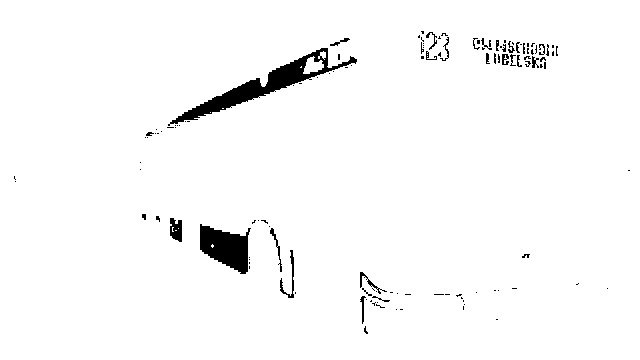
\includegraphics[width=0.9\textwidth]{img/exp_hsv_threshold_number_detector}
\end{figure}

Po wykryciu potencjalnego numeru należałoby uruchomić drugi stopień
kaskady, który stwierdzałby czy dany fragment rzeczywiście reprezentuje
numer.

Niestety niepewność związana z~niepożądanym wykrywaniem przypadkowych
pomarańczowych numerów i~dyskryminacją pasażerów, którzy
poruszają się autobusami z~zielonymi wyświetlaczami skutecznie
zniechęciła do implementacji rzeczonego rozwiązania.

Na tym etapie dodatkowym argumentem było niepożądane 
pominięcie w~ten sposób
wszystkich autobusów z~tabliczkami gdzie numer zapisywany jest czarną
czcionką na białym tle. Argument ten był jeszcze wtedy aktualny, choć
ostatecznie zrezygnowano z~wykrywania frontów tzw. ,,starego typu'' -
Ikarus, Jelcz Berliet itp. Zostało to pośrednio wymuszone przez 
znacznie mniejszą skuteczność uniwersalnego detektora, który był
wyszkolony przy użyciu frontów z~tabliczkami i~tych z~wyświetlaczami, 
o~czym szerzej w~jednym z~następnych podrozdziałów.

\subsection{Tesseract}

Pierwsza próba z~narzędziem Tesseract okazała się bardzo obiecująca.
Ręcznie wycięty fragment reprezentujący numer 140 został podany 
jako argument wywołania komendy \verb|tesseract|:

\lstinputlisting{data/tesseractcommand.txt}

Parametr \verb|-psm 8| określał metodę segmentacji obrazu jako ,,jedno
słowo''. Obraz wejściowy \verb|nuber.png| został zaprezentowany
na rusunku poniżej. Wynik jaki otrzymano dla powyższego doświadczenia
był wzorowy - w~pliku wynikowym \verb|out.txt| pojawił
się ciąg znaków: 140.

\begin{figure}[h!]
    \caption{Pierwszy numer testowy - prawidłowo odczytany}
    \centering
    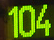
\includegraphics[width=0.25\textwidth]{img/exp_number_01}
\end{figure}

Szereg kolejnych doświadczeń przyniósł jednak rozczarowanie. 
Wiele dobrze widocznych numerów w~stosunkowo wysokiej rozdzielczości 
nie została odczytana w~ogóle (ciąg znaków zerowej długości). Zdarzały 
się nawet przypadki kiedy trzycyfrowy numer został rozszyfrowany jako
kilka wielocyfrowych liczb (ciąg ze spacjami).


\begin{table}[h!]
  \centering
  \begin{tabular}{c l c l c l}
    Obraz1 & Odczyt1 & Obraz2 & Odczyt2 & Obraz3 & Odczyt3  \\ 
    \begin{minipage}{.2\textwidth}
      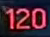
\includegraphics[width=\textwidth]{img/exp_number_02}
    \end{minipage}
    &
    120
    &
    \begin{minipage}{.2\textwidth}
      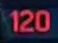
\includegraphics[width=\textwidth]{img/exp_number_03}
    \end{minipage}
    &
    120.
    &
    \begin{minipage}{.2\textwidth}
      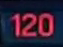
\includegraphics[width=\textwidth]{img/exp_number_04}
    \end{minipage}
    &
    120
    \\
    \begin{minipage}{.2\textwidth}
      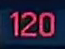
\includegraphics[width=\textwidth]{img/exp_number_05}
    \end{minipage}
    &
    120
    &
    \begin{minipage}{.2\textwidth}
      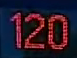
\includegraphics[width=\textwidth]{img/exp_number_06}
    \end{minipage}
    &
    120
    &
    \begin{minipage}{.2\textwidth}
      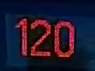
\includegraphics[width=\textwidth]{img/exp_number_07}
    \end{minipage}
    &
    120
    \\ 
  \end{tabular}
  \caption{Wyniki pierwszej serii testowej tesseract}\label{tbl:tess_01}
\end{table}

Niestety w~momencie pisania tego tekstu wyniki pierwotnych eksperymentów
zostały utracone. Mając już gotową implementacją opartą na innym
rozwiązaniu wykonano dwie krótkie serie próbne, których wyniki
zamieszczono w~tabelkach poniżej.

Pierwsza seria próbna pokazuje, że rozwiązanie oparte na narzędziu
tesseract ma duży potencjał i~wysokie prawdopodobieństwo powodzenia.
Jednak aby zobrazować problemy jakie niesie ze sobą to podejście
wykonano dwie kolejne, celowo nieudane próby.

\begin{table}[h!]
  \centering
  \begin{tabular}{c l c l}
    Obraz1 & Odczyt1 & Obraz2 & Odczyt2  \\ 
    \begin{minipage}{.2\textwidth}
      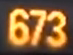
\includegraphics[width=\textwidth]{img/exp_number_n01}
    \end{minipage}
    &
    673
    &
    \begin{minipage}{.2\textwidth}
      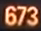
\includegraphics[width=\textwidth]{img/exp_number_n02}
    \end{minipage}
    &
    673
     
    \\ 

    \begin{minipage}{.2\textwidth}
      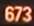
\includegraphics[width=\textwidth]{img/exp_number_n03}
    \end{minipage}
    &
    673
    &
    \begin{minipage}{.2\textwidth}
      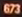
\includegraphics[width=\textwidth]{img/exp_number_n04}
    \end{minipage}
    &
    .

    \\ 

  \end{tabular}
  \caption{Wyniki drugiej serii testowej tesseract}\label{tbl:tess_02}
\end{table}

W~drugiej serii przedstawiono zależność skuteczności tesseracta od 
rozdzielczości obrazu, gdzie czwarty obraz został zinterpretowany
jako kropka. Poziom dokładności jest w~tym przypadku na poziomie
jak najbardziej akceptowalnym. Trudno nawet spodziewać się lepszego
wyniku.

Największe wątpliwości
co do wykorzystania tesseracta w~rozwiązaniu docelowym zostały zobrazowane
przez wyniki trzeciej serii testowej. Tutaj zniekształcenia spowodowane
refleksami pojawiającymi się na szybie osłaniającej wyświetlacz
zupełnie uniemożliwiły skuteczne odczytanie numeru.

\begin{table}[h!]
  \centering
  \begin{tabular}{c l c l c l}
    Obraz1 & Odczyt1 & Obraz2 & Odczyt2 & Obraz3 & Odczyt3  \\ 
    \begin{minipage}{.2\textwidth}
      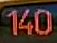
\includegraphics[width=\textwidth]{img/exp_number_f01}
    \end{minipage}
    &
     26
    &
    \begin{minipage}{.2\textwidth}
      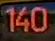
\includegraphics[width=\textwidth]{img/exp_number_f02}
    \end{minipage}
    &
    170
    &
    \begin{minipage}{.2\textwidth}
      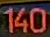
\includegraphics[width=\textwidth]{img/exp_number_f03}
    \end{minipage}
    &
    140
    \\
    \begin{minipage}{.2\textwidth}
      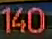
\includegraphics[width=\textwidth]{img/exp_number_f04}
    \end{minipage}
    &
     9.
    &
    \begin{minipage}{.2\textwidth}
      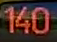
\includegraphics[width=\textwidth]{img/exp_number_f05}
    \end{minipage}
    &
    
    &
    \begin{minipage}{.2\textwidth}
      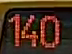
\includegraphics[width=\textwidth]{img/exp_number_f06}
    \end{minipage}
    &
    
    \\
    \begin{minipage}{.2\textwidth}
      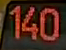
\includegraphics[width=\textwidth]{img/exp_number_f07}
    \end{minipage}
    &
     1420.
    &
    \begin{minipage}{.2\textwidth}
      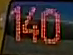
\includegraphics[width=\textwidth]{img/exp_number_f08}
    \end{minipage}
    &
     711913
    &

  \end{tabular}
  \caption{Wyniki trzeciej serii testowej tesseract}\label{tbl:tess_03}
\end{table}

Dodatkowym problemem jest prawdopodobna tendencja do nadinterpretacji
przy odczycie numerów gdy rozdzielczość jest już na tyle wysoka, że
widoczne są poszczególne diody - ostatni obraz z~serii trzeciej.
Rozwiązaniem tego problemu byłoby zastosowanie adaptacyjnego filtru
Gaussa lub operacji morfologicznych, np.: otwarcia + zamknięcia.
Opór przed tego typu zabiegami spowodowany brakiem narzędzi 
do mierzenia skuteczności zaowocował pominięciem narzędzi tesseract
w~rozwiązaniu końcowym. Tym nie mniej jest to metoda z~największym
potencjałem spośród omawianych do tej pory ,,ślepych uliczek''. 
Fakt, że w~trzech powyższych próbach dwie z~nich dały wynik pozytywny
i~to bez wcześniejszej konfiguracji narzędzia (nauka dodatkowych
krojów czcionek itp.) świadczy, że można z~powodzeniem próbować
usprawnić proponowane w~tym opracowaniu rozwiązanie poprzez 
podmianę ostatniego (trzeciego) kroku kaskady w~oparciu o~bibliotekę
tesseract. Tym bardziej, że wspomniana biblioteka posiada gotową
implementację działającą na systemie android.

\subsection{MSER - lokalizacja numeru}

Ostatnim eksperymentem, którego wyniki nie były dostatecznie przekonujące
do użycia badanej metody w~rozwiązaniu docelowym, było
wykorzystanie algorytmu MSER (\textit{ang. Most Stable Extreme Regions})
do określania położenia numeru.

\begin{figure}[h!]
    \caption{Pierwszy numer testowy - prawidłowo odczytany}
    \centering
    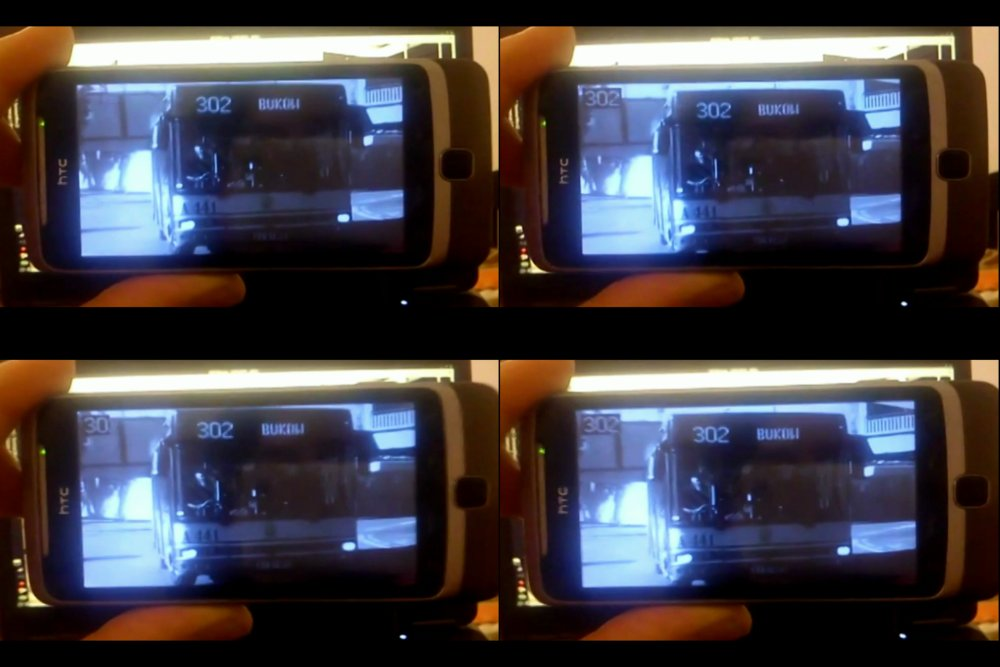
\includegraphics[width=0.9\textwidth]{img/exp_mser_concerns}
\end{figure}

Poglądowe rezultaty zostały zaprezentowane na rysunku poniżej. 
Niestety w~zależności od rozdzielczości zmieniała się podatność
numeru na wykrycie. Dla niewielkich rozdzielczości numer był rozpoznawany
jedynie jako całość, gdzie ograniczeniem geometrycznym wykorzystanym
do tego celu był prostokąt pocztówkowy o~proporcjach 2 na 3 - prezentowany
przykład. Na lewym dolnym obrazie można zaobserwować wykrycie jedynie
pierwszych dwóch cyfr numeru.

W~wyższych rozdzielczościach aby zachować wprowadzone ograniczenie
niezbędne było zastosowanie filtru rozmywającego. Bez filtru
wykrywane regiony reprezentowały poszczególne cyfry składowe numeru.
W~tym przypadku ograniczenie geometryczne wahało się od 1x4 (pionowy
prostokąt) dla jedynki do 2x3 (również prostokąt ustawiony pionowo) dla
pozostałych cyfr.

Zbyt duża liczba czynników wpływających na skuteczność:
\begin{itemize}
    \item krój czcionki: wysokie, wąskie,
    \item inne ograniczenia geometryczne dla zmiennej ilości cyfr
        w~numerze,
    \item stosowanie adaptacyjnych filtrów celem rozmycia obrazów
        w~wyższych rozdzielczościach (autobus bliżej obserwatora),
    \item stosowanie dwóch niezależnych detektorów, oddzielnie dla
        cyfr i~oddzielnie dla numerów.
\end{itemize}

spowodowały, że pominięto tę metodę w~rozwiązaniu końcowym.
Tym nie mniej jest to druga (po narzędziu tesseract) metoda, której
wyniki były na tyle obiecujące, że przemyślana implementacja
mogłaby z~powodzeniem zastąpić ostatecznie wykorzystany kaskadowy
detektor haara (lub jak kto woli pomysłu panów Violi i Jonesa).


\section{Eksperymenty częściowo udane}

W~podrozdziale tym przedstawione i~omówione zostały doświadczenia
związane z~algorytmami, narzędziami i~bibliotekami wykorzystanymi
w~ostatecznym programie. Pierwsze opisy powstawały równolegle
do toczących się prac więc są raczej nieporadnym sprawozdaniem
niż rzetelną analizą za co serdecznie przepraszam.

Dodatkowo wprowadzony został logiczny podział na pięć etapów:

\begin{enumerate}
    \item Przygotowanie zbioru uczącego, który miał być jednocześnie
        zbiorem testowym. Pierwsza wersja przygotowanego zbioru
        faktycznie mogła posłużyć za zbiór testowy. Składał się
        bowiem z~pełnych klatek w~których oznaczone były wystąpienia
        frontów - osobny plik tekstowy ze współrzędnymi. Ostateczna
        wersja przechowywanych danych ograniczała się do wycinków
        zawierających tylko szukane obiekty - oszczędność przestrzeni
        dyskowej. Co w~pewnym stopniu fałszowało wyniki. Funkcja
        gorzej radziła sobie z~wyszukiwaniem obiektów, które nie
        zawierały dostatecznego marginesu, najlepiej o~szerokości
        zbliżonej do rozmiarów samego obiektu.
    \item Wstępna segmentacja - wyszukiwanie frontu autobusu, wraz
        z~dodatkową analizą wpływu zadanych parametrów na skuteczność
        szkolonego detektora.
    \item Wyłuskanie fragmentu obrazu zawierającego wyłącznie numer -
        kaskadowy detektor wykrywający numery.
    \item Dziesięć detektorów wykrywających cyfry i~ich wykorzystanie
        w~celu zawężenia obszaru poszukiwań w~procesie dopasowywania 
        wzorca (\textit{ang. Template Matching}), który to proces
        jest najbardziej intensywny obliczeniowo z~użytych.
    \item Krótkie testy związane ze skutecznością i~zasadnością
        wykorzystania metody \textit{Template Matching} w~celu weryfikacji
        potencjalnych obszarów reprezentujących cyfry.
\end{enumerate}

Pierwszy etap pochłonął najwięcej czasu. Podjęte zostały próby 
przygotowania procedury i~oprogramowania wspomagających określenie
skuteczności implementowanych rozwiązań oraz określenia 
najbardziej optymalnych parametrów do wykorzystania podczas procesu
uczenia detektora narzędziem z~pakietu OpenCV: \verb|train_cascade|.

O~ile skuteczność znajdowania frontów autobusów - wstępna segmentacja - 
jest kluczowa dla poprawnego funkcjonowania projektowanego programu 
i~zasadnym jest jej rzetelne przetestowanie to skuteczność pozostałych
etapów - ze względu na zastosowane ograniczenia - nie jest już tak
istotna (o~czym więcej w~następnym rozdziale). Pewnym usprawiedliwieniem
i~w~pewnym sensie powodem nie przetestowania wszystkich parametrów
wejściowych narzędzia do szkolenia detektorów był czas ich szkolenia 
- od jednej do kilkunastu godzin, dla detektora cech LBP. Ostatecznie
celem nie była analiza samych narzędzi a~opracowanie i~implementacja
skutecznego programu do odczytywania numerów nadjeżdżających autobusów.

\subsection{Zbiór danych uczących i testowych}

Dane wykorzystane do procesu uczenia detektorów frontów autobusów
składają się z~dwóch części.

Pierwszą partią danych ucząco-testowych było 11 zestawów obrazów
przygotowanych z~uprzednio pobranych filmów z~serwisu YouTube.
Każdy zestaw składał się z co najmniej dwóch zbiorów. Obrazów 
reprezentujących oznaczone fronty autobusów oraz obrazów tła
(ang. background). Opcjonalnym zbiorem był zestaw oznaczonych 
frontów autobusów typu Solaris. Osobny zestaw frontów miał na celu
porównanie skuteczności detektorów przygotowanych tylko przy pomocy
pojedynczego typu obiektu oraz tych do przygotowania których użyto
obiektów znacząco od siebie różnych.

Drugi zestaw to obrazy pobrane z~serwisu \verb|http://www.phototrans.eu/|.
Zbiór ten zawiera 9067 kwadratowych wycinków różnych rozmiarów
przedstawiających wyłącznie fronty autobusów. Ze względu na mnogość
typów i~nieusystematyzowanie zbioru jego szczegółowy opis nie będzie
zamieszczony. Ze względu na specyfikę skryptu pobierającego zdjęcia
z~serwisu zostały ułożone zgodnie z~kolejnością linii autobusowych.
Kolejność jest pseudo alfabetyczna, gdzie w~pierwszej kolejności
są numery jednocyfrowe, potem kolejno dwu i~trzycyfrowe. Poza tym 
nie ma żadnej systematyczności.

Poniżej zamieszczono szczegółowy opis części pierwszej zbioru.
Podział na autobusy Solaris i Inne okazał się nietrafiony. 
W~naturalny sposób podczas uczenia detektorów zidentyfikowany został 
inny podział o~czym w~kolejnych rozdziałach.

\subsubsection{Zbiór jJ9ixBfVR5k}

W~zbiorze znalazły się następujące typy autobusów: 
\begin{itemize}
    \item Jelcz: M121M (x:3,y:1), M121CNG (x:4,y:1),
    \item Ikarus 280 (x:1, y:1),
    \item Man: NL223 (x:2, y:[1:2]), (x:3, y:2 - zielony wyświetlacz),
        Lion's City (x:4, y:2),
    \item Scania OmniCity CN (x:1, y:2). 
\end{itemize}
Współrzędne w~nawiasach określają pozycję modelu autobusu na rysunku
\ref{fig:jJ9ixBfVR5k_types}.
Jaden z modeli autobusów Man został wyposażony w zielony wyświetlacz numeru.
Jet to bardzo trudny przypadek w kontekście rozpoznawania numeru.

\begin{figure}[!h]
    \centering
    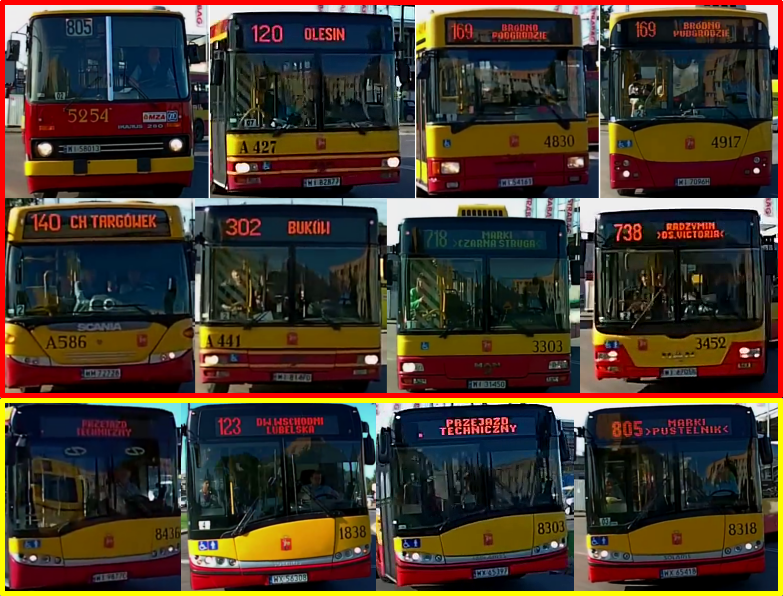
\includegraphics[width=0.9\textwidth]{img/exp_trainig_data_jJ9}
    \caption{Typy autobusów zawarte w zbiorze jJ9ixBfVR5k}
    \label{fig:jJ9ixBfVR5k_types}
\end{figure}

Liczebność zebranych próbek została przedstawiona w~tabelce nr. 
\ref{tab:jJ9ixBfVR5k_count}.

\begin{table}[!h]
    \centering
    \begin{tabular}{c|c|c}
        Front   & Solaris   & Background \\ \hline
        2587    & 222       & 2239
    \end{tabular}
    \caption{Liczebność zbioru jJ9ixBfVR5k}
    \label{tab:jJ9ixBfVR5k_count}
\end{table}

\newpage

\subsubsection{Zbiór vYqZ4-tH4M0}

W~zbiorze znalazły się te same dwa modele autobusu Jelcz co w~zbiorze
poprzednim. Powtórzyły się także modele: Ikarus, Scania oraz dwa modele
autobusów Man. Dodatkowo pojawił się model: Mercedes Citaro, oraz trzy 
niezidentyfikowane bliżej modele - pozycje: druga, trzecia i~czwarta 
w~rzędzie drugim na rysunku \ref{fig:vYqZ4-tH4M0_types} 
(prawdopodobnie Solaris, Autosan oraz Jelcz).

\begin{figure}[!h]
    \centering
    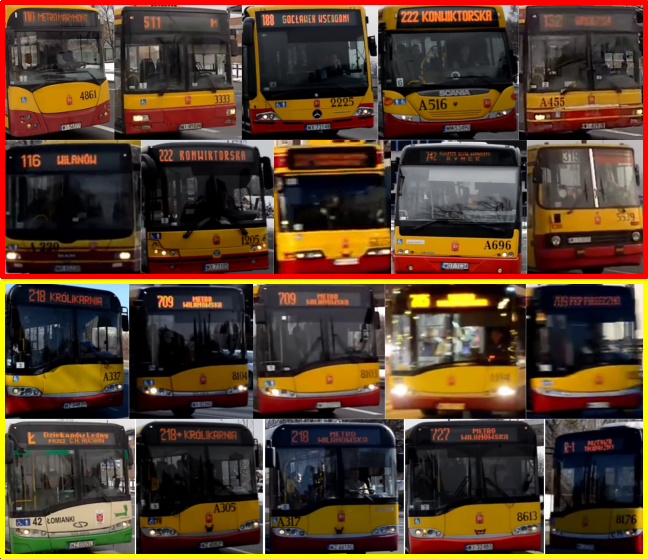
\includegraphics[width=0.9\textwidth]{img/exp_trainig_data_vYq}
    \caption{Typy autobusów zawarte w zbiorze vYqZ4-tH4M0}
    \label{fig:vYqZ4-tH4M0_types}
\end{figure}

Jeżeli chodzi o~liczebność to podzbiór ten plasuje się w~środku 
zestawienia.
Dokładne dane zamieszczono w~tabeli \ref{tab:vYqZ4-tH4M0_count}.

\begin{table}[!h]
    \centering
    \begin{tabular}{c|c|c}
        Front   & Solaris   & Background \\ \hline
        291     & 320       & 230 
    \end{tabular}
    \caption{Liczebność zbioru vYqZ4-tH4M0}
    \label{tab:vYqZ4-tH4M0_count}
\end{table}

\newpage

\subsubsection{Zbiór J8h8j6096Uw}

W~zbiorze zabrakło zdjąć reprezentujących fronty autobusów marki
Solaris. Znalazły się natomiast dwa modele marki Man - wersja 
z~,,płaską'' maską (NL223) oraz model z~charakterystycznym czarnym
wgłębieniem w~centralnej jej części (Lion's City).

\begin{figure}[!h]
    \centering
    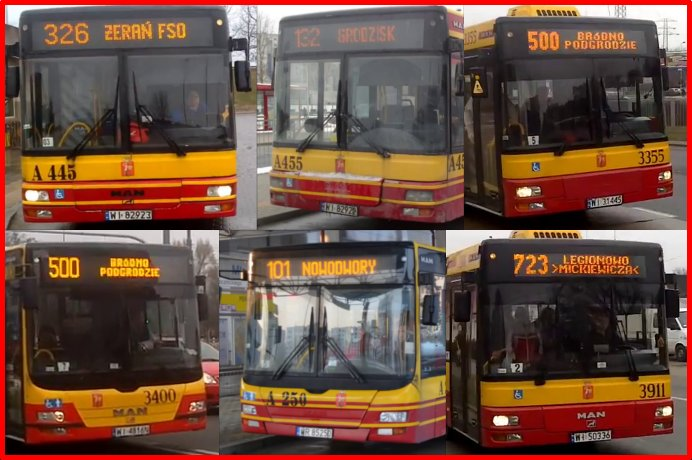
\includegraphics[width=0.65\textwidth]{img/exp_trainig_data_J8h}
    \caption{Typy autobusów zawarte w zbiorze J8h8j6096Uw}
    \label{fig:J8h8j6096Uw_types}
\end{figure}

\begin{table}[!h]
    \centering
    \begin{tabular}{c|c|c}
        Front   & Solaris   & Background \\ \hline
        182     & brak      & 427 
    \end{tabular}
    \caption{Liczebność zbioru J8h8j6096Uw}
    \label{tab:J8h8j6096Uw_count}
\end{table}

\subsubsection{Zbiór aO71uxrP9B0}

W~zbiorze miejsce znalazły zaledwie dwa modele autobusu Volvo plus 
występujący już wcześniej Mercedes Citaro.

\begin{figure}[!h]
    \centering
    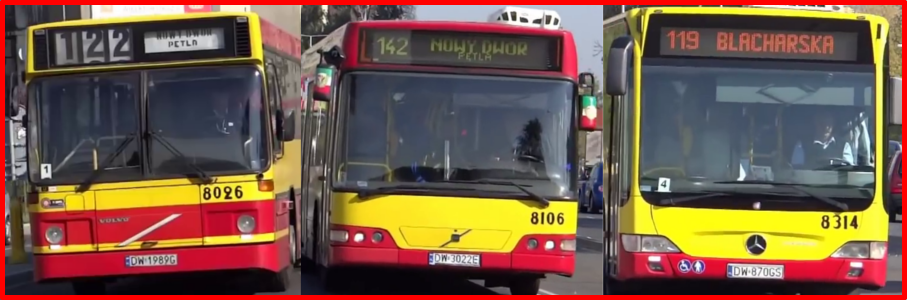
\includegraphics[width=0.65\textwidth]{img/exp_trainig_data_aO7}
    \caption{Typy autobusów zawarte w zbiorze aO71uxrP9B0}
    \label{fig:aO71uxrP9B0_types}
\end{figure}

\begin{table}[!h]
    \centering
    \begin{tabular}{c|c|c}
        Front   & Solaris   & Background \\ \hline
        177     & brak      & 977 
    \end{tabular}
    \caption{Liczebność zbioru aO71uxrP9B0}
    \label{tab:aO71uxrP9B0_count}
\end{table}

\newpage

\subsubsection{Zbiór J6sD0Tc2Dbs}

Zbiór ten zawiera dwa rodzaje autobusów marki Man oraz dwie wersje autobusu
Solaris - ze znaczkiem na masce oraz bez niego (maska gładka). Wyświetlacze
prezentujące numer wykorzystane w~przedstawionych modelach Solarisów
skutecznie uniemożliwiają odczytanie go przez jakiekolwiek urządzenie. 
Nawet człowiek nie jest w~stanie domyślić się numeru który został utrwalony
na zdjęciach - rysunek \ref{fig:J6sD0Tc2Dbs_types}. Historyczne modele
skody zostały zaprezentowane w~ramach ciekawostki i~nie będą uwzględniane
w~dalszych eksperymentach.

\begin{figure}[!h]
    \centering
    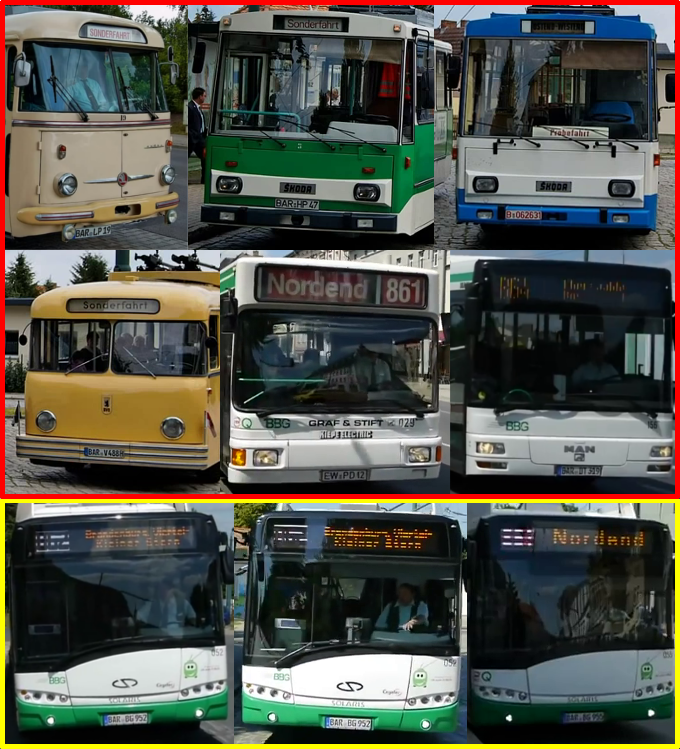
\includegraphics[width=0.65\textwidth]{img/exp_trainig_data_J6s}
    \caption{Typy autobusów zawarte w zbiorze J6sD0Tc2Dbs}
    \label{fig:J6sD0Tc2Dbs_types}
\end{figure}

\begin{table}[!h]
    \centering
    \begin{tabular}{c|c|c}
        Front   & Solaris   & Background \\ \hline
        156     & 124       & 203 
    \end{tabular}
    \caption{Liczebność zbioru J6sD0Tc2Dbs}
    \label{tab:J6sD0Tc2Dbs_count}
\end{table}

\newpage

\subsubsection{Zbiór IHarVPkXwSg}

W~zbiorze - podobnie jak poprzednio - znalazły się autobusy zabytkowe.
Modele w~rzędzie pierwszym (dotyczy pozycji pierwszej i~drugiej) nie 
będą wykorzystane w~dalszych eksperymentach. Mają na celu uzmysłowienie
stopnia złożoności problemu oraz fakt, że w~zależności od modelu pozycja
numeru może oscylować w~ramach górnej połowy obszaru zidentyfikowanego
jako front autobusu. Pozostałe modele, czyli
dwa modele Jelcza, Mercedes i~(prawdopodobnie, jakiś) model Mana tworzą
grupę frontów ,,różnych''. W~skład zbioru wchodzą też dwa typy autobusu
solaris - różne kształty maski.

\begin{figure}[!h]
    \centering
    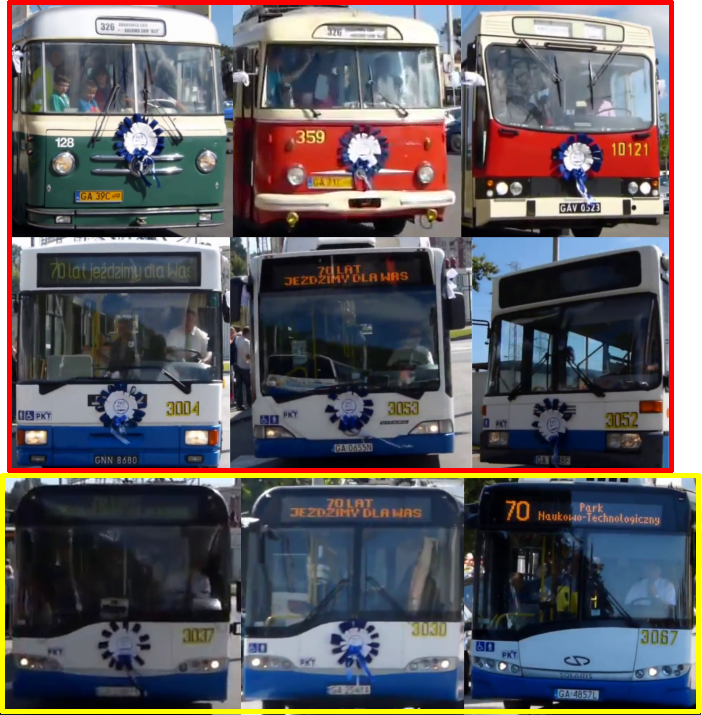
\includegraphics[width=0.8\textwidth]{img/exp_trainig_data_IHa}
    \caption{Typy autobusów zawarte w zbiorze IHarVPkXwSg}
    \label{fig:IHarVPkXwSg_types}
\end{figure}

\begin{table}[!h]
    \centering
    \begin{tabular}{c|c|c}
        Front   & Solaris   & Background \\ \hline
        342     & 172       & 1510
    \end{tabular}
    \caption{Liczebność zbioru IHarVPkXwSg}
    \label{tab:IHarVPkXwSg_count}
\end{table}

\subsubsection{Zbiór BJZLDmYMFvo}

Zbiór zawiera jedynie dwa modele autobusu Man, jednego
Jelcza i Solarisa. Jedyna uwaga może tyczyć trudności w~odczytywaniu
numeru z~autobusu man/jelcz z~wyświetlaczem w~kolorze zielonym. O~ile
warunki oświetleniowe są dobre - jak na rysunku \ref{fig:BJZLDmYMFvo_types}
- widoczność, a~co za tym idzie rozpoznawalność numeru powinna być na 
zadowalającym poziomie.

\begin{figure}[!h]
    \centering
    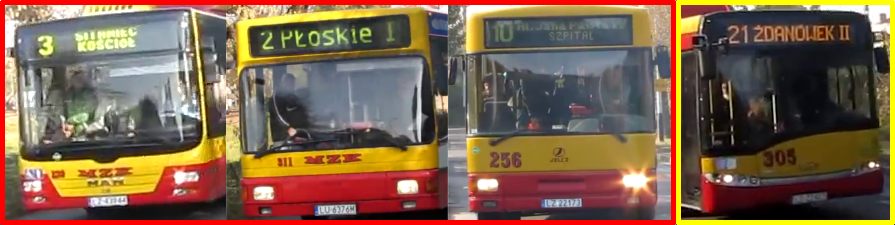
\includegraphics[width=0.95\textwidth]{img/exp_trainig_data_BJZ}
    \caption{Typy autobusów zawarte w zbiorze BJZLDmYMFvo}
    \label{fig:BJZLDmYMFvo_types}
\end{figure}

Zbiór ten posiada drugą co do wielkości 
liczbę obrazów tła w~pierwszej części. 

\begin{table}[!h]
    \centering
    \begin{tabular}{c|c|c}
        Front   & Solaris   & Background \\ \hline
        373     & 8         & 2356
    \end{tabular}
    \caption{Liczebność zbioru BJZLDmYMFvo}
    \label{tab:BJZLDmYMFvo_count}
\end{table}

\subsubsection{Zbiór \_43HUVkrA7E}

Zbiór składający się głównie ze zdjęć zawierających oznaczone fronty
zabytkowego już autobusu Jelcz Berliet. Jeżeli chodzi o~liczebność to 
główną wartością dodaną są obrazy reprezentujące tło.

\begin{figure}[!h]
    \centering
    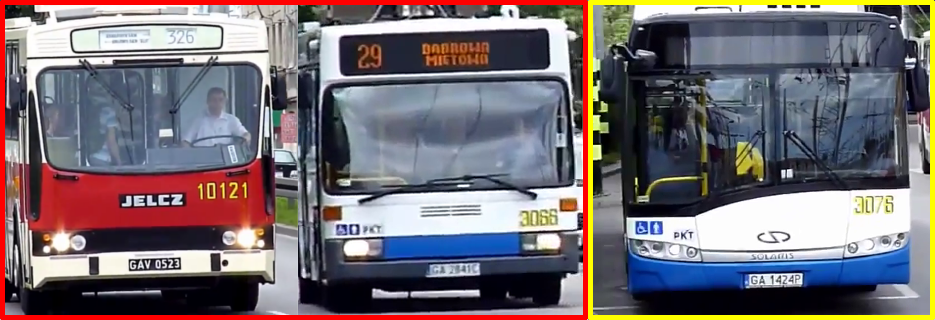
\includegraphics[width=0.75\textwidth]{img/exp_trainig_data__43}
    \caption{Typy autobusów zawarte w zbiorze \_43HUVkrA7E}
    \label{fig:_43HUVkrA7E_types}
\end{figure}

\begin{table}[!h]
    \centering
    \begin{tabular}{c|c|c}
        Front   & Solaris   & Background \\ \hline
        44      & 5         & 197 
    \end{tabular}
    \caption{Liczebność zbioru \_43HUVkrA7E}
    \label{tab:_43HUVkrA7E_count}
\end{table}

\subsubsection{Zbiór 8wdvLn40CTk}

Najmniejszy zbiór w~kontekście różnorodności zawartych modeli. Z~drugiej
strony ogromna ilość obrazów tła i~całkiem sporo oznaczonych ujęć.

\begin{figure}[!h]
    \centering
    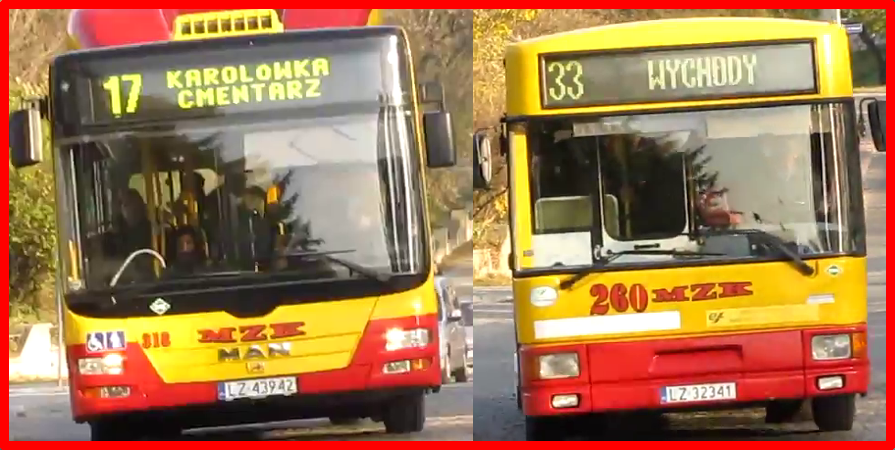
\includegraphics[width=0.45\textwidth]{img/exp_trainig_data_8wd}
    \caption{Typy autobusów zawarte w zbiorze 8wdvLn40CTk}
    \label{fig:8wdvLn40CTk_types}
\end{figure}

\begin{table}[!h]
    \centering
    \begin{tabular}{c|c|c}
        Front   & Solaris   & Background \\ \hline
        336     & brak      & 3572
    \end{tabular}
    \caption{Liczebność zbioru 8wdvLn40CTk}
    \label{tab:8wdvLn40CTk_count}
\end{table}

\subsubsection{Zbiór 75Dz6s7S-Tg}

Kolejny niewielki zbiór. Te same modele autobusu Man co w~zestawie
pierwszym. Dodatkowo dwie wersje kolorystyczne (wyświetlacz) modelu
Mercedes Citaro. Na koniec wystąpienie modelu Solaris niestety zaledwie
w~dwóch egzęplażach.

\begin{figure}[!h]
    \centering
    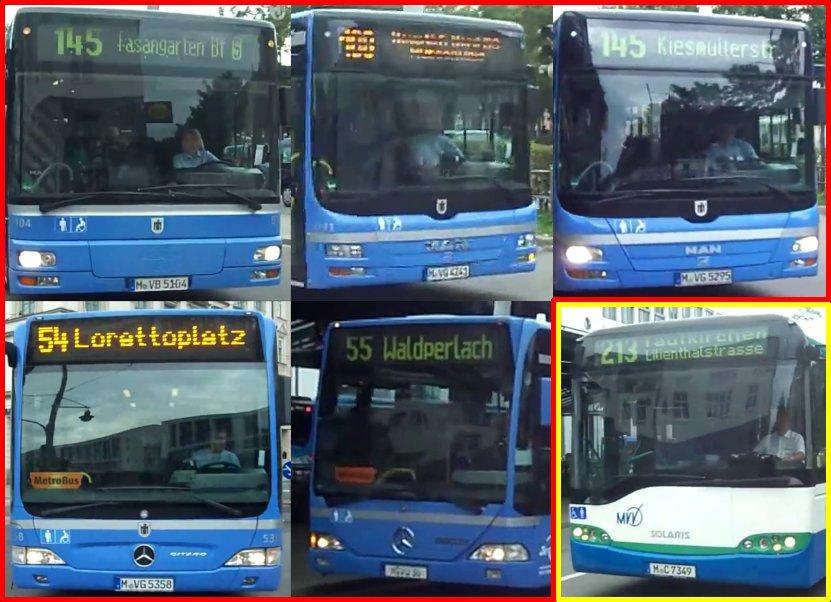
\includegraphics[width=0.75\textwidth]{img/exp_trainig_data_75D}
    \caption{Typy autobusów zawarte w zbiorze 75Dz6s7S-Tg}
    \label{fig:75Dz6s7S-Tg_types}
\end{figure}

\begin{table}[!h]
    \centering
    \begin{tabular}{c|c|c}
        Front   & Solaris   & Background \\ \hline
        81      & 2         & 179 
    \end{tabular}
    \caption{Liczebność zbioru 75Dz6s7S-Tg}
    \label{tab:75Dz6s7S-Tg_count}
\end{table}

\subsubsection{Zbiór 9hMQ4UGNxhw}

Występujące już wcześniej modele: Mercedes Citaro, zabytkowy Jelcz Berliet,
Man Lion's City, Scania OmniCity, Ikarus 280 z~ledowym wyświetlaczem,
Jelcz M121CNG (x:2, y:1). Dodatkowo dwie wersje kolorystyczne autobusu
Autosan.

\begin{figure}[!h]
    \centering
    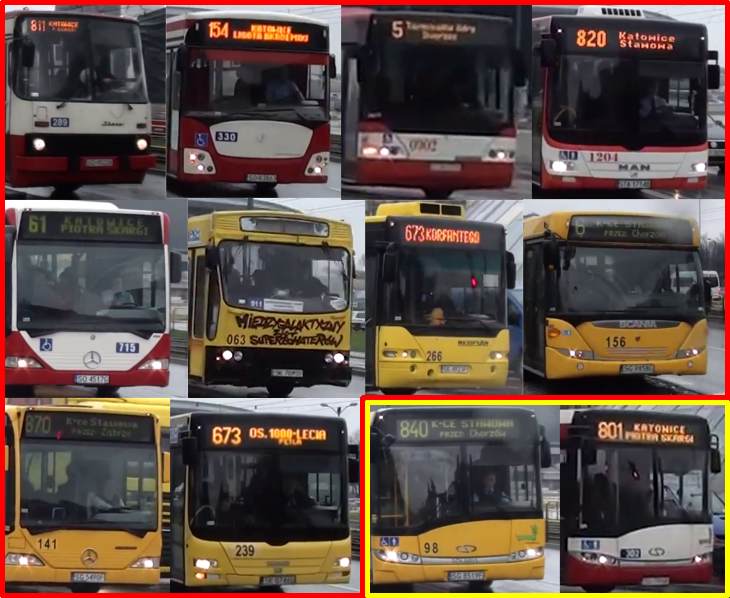
\includegraphics[width=0.95\textwidth]{img/exp_trainig_data_9hM}
    \caption{Typy autobusów zawarte w zbiorze 9hMQ4UGNxhw}
    \label{fig:9hMQ4UGNxhw_types}
\end{figure}

\begin{table}[!h]
    \centering
    \begin{tabular}{c|c|c}
        Front   & Solaris   & Background \\ \hline
        267     & 102       & 363 
    \end{tabular}
    \caption{Liczebność zbioru 9hMQ4UGNxhw}
    \label{tab:9hMQ4UGNxhw_count}
\end{table}

Ostatecznie po złączeniu wszystkich zaprezentowanych zbiorów powstały
dwa końcowe (będące jednocześnie punktem wyjścia do dalszych testów):
- zbiór wszystkich oznaczonych frontów (różne + solarisy) - 5781 sztuk,
- zbiór oznaczonych frontów autobusów typu Solaris - 955 sztuk.

Osobny zbiór zawierający tylko fronty typu Solaris miał na celu
sprawdzenie czy mnogość pozytywnych kształtów nie wpływa na skuteczność
detekcji. Stąd osobne dane uczące/testowe oraz detektor wykrywający 
tylko fronty typu Solaris. Jak się później okazało naturalny podział
- wykryty organoleptycznie, podczas oznaczania wystąpień frontów - 
wyznacza dwie grupy frontów: te z~wyświetlaczem led-owym (na całej
długości górnej krawędzi frontu) oraz te bez niego.

\subsection{Przygotowanie optymalnego detektora frontów}

Pierwsze próby związane z~procesem uczenia detektora miały na celu 
wyłonienie parametrów mających największy wpływ na skuteczność 
oraz efektywność trenowanego detektora.

\subsubsection{Porównanie detektorów HAAR, LBP i HOG}

Pierwsza iteracja uczenia detektorów miała na celu przetestowanie
opcji jakie można zadać narzędziu uczącemu - \verb|opencv_traincascade|.

Za zbiór testowy posłużył zestaw oznaczonych zdjęć oraz zdjęć tła
przygotowany dla filmu o id jJ9ixBfVR5k (charakterystyka zbioru
została opisana w~poprzednim rozdziale)

Pierwszy test miał za zadanie wyłonić najefektywniejszą metodę, do dalszych
eksperymentów. Narzędzie dostarczone wraz z~pakietem OpenCV - wspomniany
już \verb|opencv_traincascade| - pozwalał na wyszkolenie trzech
rodzajów detektorów:

\begin{itemize}
    \item detektor wykorzystujący tzw. cechy Harra - wartość 
        domyślna (HAAR),
    \item detektor LBP,
    \item detektor HOG.
\end{itemize}

Gdy jeszcze nie wszystkie wyłuskane zdjęcia były opisane, wykonany został
krótki test porównawczy skuteczności i~czasu potrzebnego na nauczenie
poszczególnych typów detektorów. Po dość chaotycznie wykonanej próbie
otrzymano następujące wyniki:

\begin{table}[!h]
\centering
\begin{tabular}{r|c|c|c|l}
    & HAAR         & LBP        & HOG              &       \\
    \hline
Solaris & 151  (43\%)  & 81  (23\%) & 61 (17\%)        & /346  \\
Różne   & 1051 (35\%)  & 748 (25\%) & 712 (24\%)       & /2925 \\
Tło     & 635  (11\%)  & 386 (6\%)  & 447 (7\%)        & /5588 \\
\end{tabular}
\caption{Porównanie skuteczności detektorów typu HAAR, LBP i HOG.}
\label{tab:haar_lbp_hog_comparison}
\end{table}

Jako, że nie wszystkie jeszcze próbki były opisane, stąd zaniżona wartość
w~ostatniej kolumnie. Łatwo jednak zaobserwować trend dokładności
tychże detektorów.

O ile skuteczność detektora w~funkcji czasu potrzebnego na jego 
wyszkolenie dla detektorów cech HAAR-a i~LBP był skorelowany i~sensowny,
to w~przypadku cech HOG było już nieco inaczej.
Detektor oparty o~cechy HAAR-a potrzebował
zdecydowanie więcej czasu na proces trenowania co miało przełożenie 
na jego skuteczność. LBP natomiast okazał się nieco mniej skuteczny
lecz jego szkolenie trwało krócej o~rząd wielkości.
Cechy HOG w~tym zestawieniu okazały się mało interesującym kandydatem
- skuteczność gorsza niż LBP przy czasie szkolenie o~wiele dłuższym.

Czasy uczenia dla poszczególnych detektorów wyglądały następująco:
\begin{itemize}
    \item HAAR - 6 godzin
    \item HOG - 3 godziny
    \item LBP - 40 min
\end{itemize}

\subsubsection{Porównanie detektorów - Solaris i frontów różnych}

Wbrew obawom detektor wyszkolony przy użyciu wszystkich frontów radził
sobie znacznie lepiej w~wykrywaniu frontów autobusów Solaris niż ten
wyszkolony z~użyciem tylko tego rodzaju frontów. Wyniki dla ustawień
domyślnych dla detektorów typu LBP przedstawiono w tabelce nr 
\ref{tab:sol_vs_all}.

\begin{table}[!h]
    \centering
    \begin{tabular}{r|c|c|l}
            & Solaris(detektor) & Wszystkie typy (detektor) &           \\
            \hline
wszystkie   & 175 (3\%)         & 3466 (71\%)               & 4836      \\
solaris     & 609 (63\%)        & 854 (89\%)                & 955       \\
błędy       & 289 (1\%)         & 56088 (310\%)             & 18048     \\
    \end{tabular}
    \caption{Skuteczność detektorów wyszkolonych tylko dla typów solaris kontra tych wyszkolonych dla wszystkich typów frontów}
    \label{tab:sol_vs_all}
\end{table}

Jak widać problemem nie jest skuteczność wykrywania istniejących obiektów
tylko ogromna liczba wyników błędnych. W~kolejnych krokach zostaną opisane
próby poradzenia sobie z~tym problemem.

\subsubsection{Parametry minHitRate i~maxFalseAlarmRate}

Niestety wraz ze zwiększaniem parametru \verb|minHitRate|
znacząco zwiększała
się liczba błędnych trafień. Poniższe wykresy przedstawiają znaczny wzrost
błędnych wyników oraz znacznie wolniejszy przyrost pozytywnych 
rezultatów.
\begin{center}
\begin{tikzpicture}
\begin{axis}[
    title=Błędne trafienia,
    ylabel={$falseAlarmHits$},
    xlabel={$minHitRate$},
    minor y tick num=1,
]
\addplot table {data/hitratio_fal.dat};
\end{axis}
\end{tikzpicture}
\end{center}

Sądząc po poniższym wykresie, poziom 80\% był jak najbardziej do
osiągnięcia. Po dodatkowym zmniejszeniu liczby fałszywych alarmów 
do akceptowalnych wartości (<20\%) detektor w~wersji deweloperskiej 
można było uznać za ukończony.

\begin{center}
\begin{tikzpicture}
\begin{axis}[
    title=Pozytywne trafienia,
    ylabel={$posotiveHits$},
    xlabel={$minHitRate$},
    minor y tick num=1,
    legend style={at={(0.06,0.73)},anchor=north west}
]
\addplot table {data/hitratio_fro.dat};
\addlegendentry{wszystkie}
\addplot table {data/hitratio_sol.dat};
\addlegendentry{solaris}
\end{axis}
\end{tikzpicture}
\end{center}

Pierwsza próba zmniejszenia nieudanych trafień polegała na zmianie 
parametru \verb|maxFalseAlarmRate| podczas uczenia detektora. 
Wykonano pięć
sesji uczenia detektora dla wartości: od domyślnej 0.5 do 0.1.

Ostatecznie przy ilości próbek pozytywnych i~negatywnych 
na poziomie 5000 opisywane wyżej parametry nie miały już prawie w~cale
znaczenia. Przy domyślnych wartościach skuteczność detektora była 
zadowalająca.

\subsubsection{Podejście drugie - usuniecie zdeformowanych frontów}

Podczas oznaczania frontów autobusów nastąpiła pewnego rodzaju
nadgorliwość. Podczas wyboru klatek do późniejszego oznaczenia
wystąpienia frontu klasyfikowano wszystkie wystąpienia autobusu
czołem do kamery jako poprawne i~wartościowe. Podczas gdy autobus
był ustawiony prostopadle do matrycy aparatu klatka taka była
jak najbardziej poprawna i~zawarte w~niej informacje mogły
z~powodzeniem być wykorzystane podczas uczenia detektora. Jednak
gdy kąt między osią autobusu, a~płaszczyzną matrycy był mniejszy
niż 45 stopni, zdjęcie nie niosło ze sobą informacji przydatnych
w~procesie uczenia. Po pierwsze numer autobusu był już wtedy
niewidoczny - informacja została utracona. Po drugie wprowadzone
zostało zbędne zaburzenie w~wyglądzie szukanych obiektów,
które mogłoby niekorzystnie wpłynąć na skuteczność wyszkolonych
w~ten sposób detektorów.

W~ramach drugiej iteracji poszukiwania optymalnego detektora
usunięto wszystkie oznaczenia frontu pasujące do opisu
z~poprzedniego akapitu. Kilka takich przypadków można
zaobserwować na zdjęciu poniżej.

\begin{figure}[h!]
    \centering
    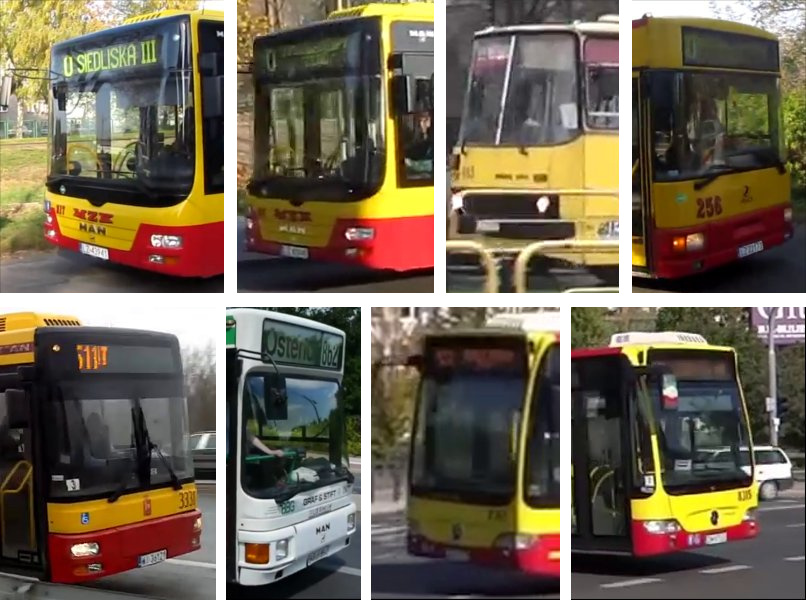
\includegraphics[width=0.8\textwidth]{img/exp_removed_distorted_fronts}
    \caption{Usunięte oznaczenia ze względu na zniekształcenia geometryczne}
\end{figure}

Jednak zanim przejdziemy do weryfikacji skuteczności poprawionego
zbioru, przedstawione zostanie porównanie skuteczności już nauczonych
detektorów. W~poprzednich podrozdziałach (bardzo chaotycznie) opisane
zostały pierwsze próby utworzenia optymalnego detektora. W~ramach
tych eksperymentów powstało 15 plików definiujących detektory, do utworzenia
których użyto zmiennych parametrów. W~pierwszej iteracji zmianie podlegały
parametry:

\begin{itemize}
\item featureType - HAAR(default), LBP, HOG,
\item minHitRate - minimalna procentowa wartość pozytywnych wykryć (domyślnie 0.995),
\item maxFalseAlarmRate - maksymalna procentowa wartość błędów (domyślnie 0.5),
\item numNeg - liczba obrazów tła do wykorzystania.
\end{itemize}

Dodatkowo powstały dwa detektory LBP osobno dla frontów typu solaris i~dla
całości zbioru (5690 wystąpień). Oto cała lista plików z~pierwszej iteracji:

\begin{enumerate}
\item dev\_01\_haar\_default.xml
\item dev\_02\_lbp\_default.xml
\item dev\_03\_hog\_default.xml
\item dev\_04\_lbp\_solaris\_943.xml
\item dev\_05\_lbp\_all\_5690.xml
\item dev\_06\_lbp\_all\_posratio\_996.xml
\item dev\_07\_lbp\_all\_posratio\_997.xml
\item dev\_08\_lbp\_all\_posratio\_998.xml
\item dev\_09\_lbp\_all\_posratio\_999.xml
\item dev\_10\_lbp\_all\_posratio\_999\_maxfalse\_04.xml
\item dev\_11\_lbp\_all\_posratio\_999\_maxfalse\_03.xml
\item dev\_12\_lbp\_all\_posratio\_999\_maxfalse\_02.xml
\item dev\_13\_lbp\_all\_posratio\_999\_maxfalse\_01.xml
\item dev\_14\_lbp\_all\_posratio\_999\_numneg\_2000.xml
\item dev\_15\_lbp\_all\_posratio\_999\_numneg\_4000.xml
\end{enumerate}

Pierwsze trzy pliki utworzone były na ograniczonym podzbiorze danych, gdyż
nie wszystkie próbki były wtedy opisane.

Procedura porównywania skuteczności operowała na zbiorze obrazów
reprezentujących wystąpienia frontów autobusów solaris połączonym
z~ogólnym zbiorem. Poprawne
wykrycie liczone było wtedy gdy współrzędne prostokątów wykrytego
i~oznaczonego znajdowały się w~odległości nie większej niż 25\% odpowiadającego
wymiaru prostokąta oznaczonego: dla odciętych i~rzędnych odpowiednio szerokość
i~wysokość prostokąta. Do zliczania błędnych wykryć wykorzystano ten sam zbiór.
Ze względu na ograniczenie czasowe zrezygnowano z~wykorzystania zbioru
obrazów tła. Wyniki zaprezentowano na wykresie poniżej.

\begin{center}
\begin{tikzpicture}
\begin{groupplot}[group style={group size=1 by 2},
height=5cm,width=0.8\textwidth,
legend style={at={(0.03,0.93)},anchor=north west}]
\nextgroupplot
\addplot table {data/15_detectors_comparison_positive_percentage.dat};

\addlegendentry{Skutecznosc}

\nextgroupplot
\addplot table {data/15_detectors_comparison_negative_count.dat};
\addlegendentry{Bledne trafienia}
\end{groupplot}
\end{tikzpicture}
\end{center}

Jak widać wyniki w~większości przypadków oscylowały w~granicach 90\%.
W~odróżnieniu od poprzednich testów, te wykonane były na klatkach obrazu
w~oryginalnej rozdzielczości (wysokość 720p). 
Kolejnym krokiem było znalezienie
optymalnego czynnika skalującego. Innymi słowy jak bardzo można zmniejszyć
obraz wejściowy aby utrzymać wyniki na zadowalającym poziomie.

\subsubsection{Skalowanie obrazu wejściowego - podsumowanie}

W~celu zmniejszenia złożoności obliczeniowej przeprowadzone zostały
testy przy przeskalowanych klatkach wejściowych. W~tym przypadku
eksperymentowano już na urządzeniu i~większość testów wykonywana była
manualnie. Metodą prób i~błędów wyznaczono parametry dla których
osiągnięto optymalne wyniki. Ostatecznie w~wersji deweloperskiej 
programu wykorzystano następujące parametry:

\begin{itemize}
    \item każdą wejściową klatkę przeskalowywano do 140 pikseli wysokości
        z~zachowaniem proporcji,
    \item minimalne wymiary szukanego obiektu to 60x60 pikseli,
    \item maksymalne 120x120 - gdy osoba stojąca na przystanku jest tuż
        przy autobusie następuje duże zniekształcenia geometryczne
        frontu. Czworokąt okalający wyznaczający front jest nieco
        przesunięty i~metoda wykrywania numeru w~lewym górnym rogu jest
        wtedy nieskuteczna.
\end{itemize}

Krok pierwszy kaskady - zawężenie poszukiwań numeru do obszaru frontu
(tymczasowo lewego-górnego fragmentu frontu) - był na tyle skuteczny,
że dalsze usprawnienia tego elementu nie były wymagane. Zasadnym jest
natomiast przygotowanie zestawu testowego i~automatyczne 
przetestowanie skuteczności rozwiązania na zbiorze nawet 100 ręcznie
oznaczonych frontów.

Proces przygotowywania zbiorów uczących detektory był
na wpół zautomatyzowany. Pierwsze sto wystąpień oznaczone było ręcznie.
Następnie dla 100 wystąpień uczony był detektor, który wykorzystywano
do testowego oznaczania frontów w~kolejnej iteracji. Gdy detektor 
poprawnie oznaczył wystąpienie obiektu próbkę taką pomijano. Oznaczano
tylko niepoprawnie oznaczone fronty lub brak oznaczeń. Z~drugiej
strony błędne oznaczenia - fałszywe alarmy - powodowały umieszczenie
próbki w~zbiorze obrazów tła. W~ten sposób naocznie zaobserwowano 
tendencje jakie przejawiał szkolony detektor. Umożliwiało to też
korygowanie błędnych zachowań - na przykład ucinanie numerów (górnej
krawędzi autobusu). Co dało niemal perfekcyjne rezultaty. Mankamentem
tego rozwiązania jest to, że teraz trudno zmierzyć jego skuteczność.

W~procesie szkolenia detektora frontów w~opisany powyżej sposób
zaobserwowano jeden szczególny trend, który faworyzował pewne
szczególne cechy frontów z~wyświetlaczem. Podczas ostatniej iteracji
(do 5000 pozytywnych oznaczeń) zaobserwowano, że detektor
chętnie identyfikuje fronty z~diodowym wyświetlaczem zajmującym 
całą górną część frontu. Przy tak dużej liczbie oznaczeń
cechą szczególną okazał się właśnie ów wyświetlacz. Cecha ta była
na tyle istotna, że oznaczane były również fragmenty boków autobusów
z~wyświetlaczem bocznym, czy fragmenty frontów, na których wyświetlacz
nie zajmował całej długości górnej krawędzi (obrazek poniżej).

\begin{figure}[!h]
    \centering
    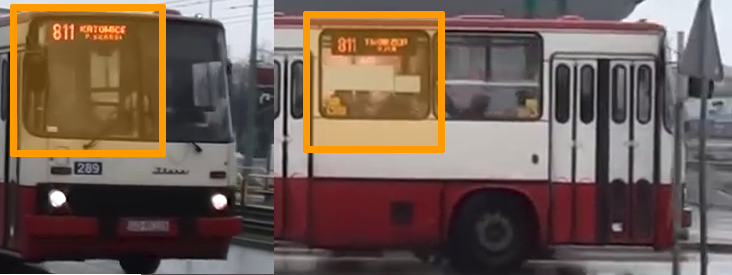
\includegraphics[width=0.95\textwidth]{img/exp_front_detector_curiosity}
    \caption{Tendencja do oznaczania fragmentów z~dużą ilością
    małych elementów w górnej części}
    \label{fig:frontdetectormorph}
\end{figure}

Możliwym rozwinięciem popełnionej implementacji jest więc przeszkolenie
detektora frontowego tak aby wykrywał również tablice boczne. Minusem
tego rozwiązania jest fakt, że z~lokalizowaniem autobusów z~tablicami
drukowanymi detektor radzi sobie znacznie gorzej. Co za tym idzie
zostały one wykluczone z~dalszych rozważań. Aby skutecznie wykrywać
fronty autobusów typu Ikarus lub starych Jelczy niezbędny byłby 
dodatkowy dedykowany detektor i~prawdopodobnie dedykowane wersje
pozostałych elementów.

\subsection{Detektor numerów}

Kaskadowy detektor wykrywający numer w~lewym górnym rogu wykrytego
frontu był jednym z~ostatnich zaimplementowanych elementów. Do wyszkolenia
detektora użyto 450 oznaczonych wystąpień numerów (jedno, dwu
i~trzycyfrowych) oraz 800 instancji tła. Ze względu na problemy podczas
szkolenia detektora dla większej liczby pozytywnych i~negatywnych 
instancji zaprzestano zwiększania ich ilości. Problem polegał na
zawieszeniu się procesu uczenia na jednym z~etapów i~gdy normalnie 
cała procedura liczona była w~dziesiątkach minut (maksymalnie 1-2 godziny)
to dla zbyt dużej liczby - w~szczególności obrazów tła proces potrafił
utknąć na danym etap na dobę.

Element ten był najsłabiej przetestowany i~wymagał usprawnienia 
w~pierwszej kolejności. Pewną formą pójścia na łatwiznę było
ograniczenie obszaru przeszukiwania do lewego górnego rogu wykrytego
frontu jak na rysunku poniżej.

\begin{figure}[!h]
    \centering
    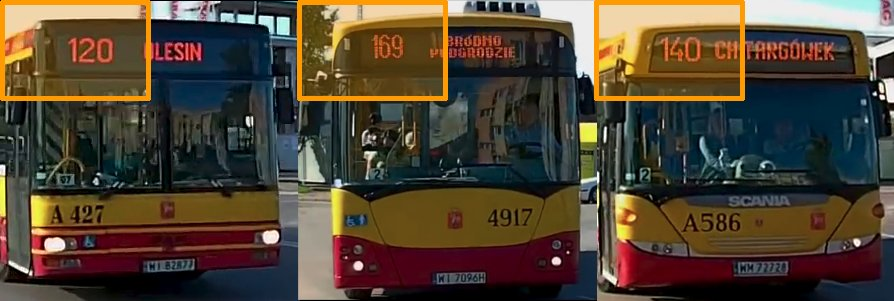
\includegraphics[width=0.95\textwidth]{img/exp_front_upper_left}
    \caption{Obszar przeszukiwany pod kątem wystąpienia numeru}
    \label{fig:frontupperleft}
\end{figure}

Możliwą alternatywą dla tego kroku jest omawiana już koncepcja
oparta na detektorze MSER.

\subsection{Detektory cyfr}

W~tym podrozdziale przedstawiona została ponowna,
niespecjalnie udana próba odnalezienia optymalnych
parametrów wejściowych na proces uczenia detektora.
W~pierwszej części przedstawiono wykresy zależności pozytywnych
i~błędnych wykryć w~zależności od ilości wykorzystanych
pozytywnych próbek w~procesie uczenia. Niestety
ogromna czasochłonność przygotowywania tego typu wykresów
była główną przyczyną zaprzestania dalszych testów.
Aby przygotować pierwszą parę wykresów wyszkolono niemal 200 detektorów.
Druga para wymagała co prawda dyle samo detektorów ale większa 
liczba użytych próbek spowodowała znaczny wzrost czasu jaki był 
potrzebny do wyszkolenia poszczególnych detektorów.

\subsubsection{Cyfra 8 - szukanie optymalnych parametrów uczenia detektora}

Pierwszą cyfrą do wykrywania której szkolono detektor była cyfra 8.
Oznaczone 513 wystąpień cyfry w~scenach i~przygotowano około 2 tysiące
obrazów tła. Przy pierwszej próbie wykorzystano 100 obrazów tła, zmienną
była natomiast liczba próbek pozytywnych, która zmieniała się w~przedziale
od 10 do 200. Wyniki w~postaci ilości wykrytych poprawnie wystąpień cyfry
8, oraz błędnych wykryć przedstawiono na wykresach poniżej.

\begin{center}
\begin{tikzpicture}
\begin{groupplot}[group style={group size=1 by 2},
height=5cm,width=0.8\textwidth,
legend style={at={(0.03,0.93)},anchor=north west}]
\nextgroupplot
\addplot table {data/digit_8_pos_10-200_neg_100_hit_ratio.dat};

\addlegendentry{Poprawne trafienia}

\nextgroupplot
\addplot table {data/digit_8-pos_10-200_neg_100_false_alarm_count.dat};
\addlegendentry{Bledne trafienia}
\end{groupplot}
\end{tikzpicture}
\end{center}

Pierwsze przekroczenie liczby 10 tysięcy błędnych wykryć odnotowano dla
liczby pozytywnych próbek równej 124. Pierwszym (prawdopodobnie przedwczesnym)
wnioskiem jest to, iż prawdopodobnie liczba obrazów tła powinna być
większa bądź równa liczbie próbek pozytywnych.

\begin{center}
\begin{tikzpicture}
\begin{groupplot}[group style={group size=1 by 2},
height=5cm,width=0.8\textwidth,
legend style={at={(0.03,0.93)},anchor=north west}]
\nextgroupplot
\addplot table {data/digit_8_pos_100-300_neg_200_hit_ratio.dat};

\addlegendentry{Poprawne trafienia}

\nextgroupplot
\addplot table {data/digit_8-pos_100-300_neg_200_false_alarm_count.dat};
\addlegendentry{Bledne trafienia}
\end{groupplot}
\end{tikzpicture}
\end{center}

Do wykonania drugiej serii testowej wykorzystano detektory
wyszkolone przy użyciu 200 obrazów tła oraz liczby pozytywnych 
próbek w~ilości od 100 do 300 obrazów. Co łatwo zauważyć liczba 
błędnych trafień zmalała niemal o~rząd wielkości. Granica 10 tysięcy
nie została przekroczona. Dla zbioru oznaczonych 500 wystąpień cyfry 
8~najlepsze detektory nie przekroczyły liczby 400 pozytywnych trafień
więc poziom skuteczności jest nieco poniżej 80\%. Jak wiadomo
do wyszkolenia końcowej wersji detektora użyto 450 pozytywnych próbek
i~800 instancji tła.

\subsubsection{Pozostałe cyfry - podsumowanie}

Podczas przygotowywania zbiorów dla pozostałych cyfr użyto 
opisanej wcześniej metody półautomatycznego wybierania próbek pozytywnych
i~negatywnych, oraz przyrostowego uczenia detektorów z~jednoczesną
weryfikacją i~korekcją rozwiązań pośrednich. Podczas całego
procesu zaobserwowano tendencje do błędnego identyfikowania cyfr pewnej
klasy przez uczone detektory i~tak:

\begin{itemize}
    \item detektor cyfry 0 miał tendencje do wykrywania instancji cyfr
        8, 6 oraz 9,
    \item detektor cyfry 5 wykrywał również cyfry 6 oraz dużo rzadziej
        cyfry 9,
    \item detektor cyfry 2 wykrywał cyfry 4 oraz 7 itd.
\end{itemize}

Największym problemem był detektor cyfry 0, który najchętniej
wykrywał inne owalne cyfry. Najpewniejszy natomiast okazał się
detektor cyfry 1. Tym nie mniej niezbędne było wprowadzenie
mechanizmu weryfikacji potencjalnie wykrytej cyfry. Stąd 
pomysł na zastosowanie dla wykrytego fragmentu obrazu metody
Template Matching.

\subsection{Template Matching}

Przeprowadzone doświadczenie miało na celu weryfikację czy
proponowana metoda sprawdzi się w~rozwiązaniu docelowym. Dla
kilku wykrytych fragmentów wywołano funkcję pakietu OpenCV 
- \verb|matchTemplate| - i~dla zwróconych obrazów wyłuskano
minimalne i~maksymalne wartości liczbowe reprezentujące trafność
dopasowania wzorca. Okazało się, że po przeskalowaniu wykrytego
fragmentu zawierającego cyfrę do określonej wysokości, zbędne
było dopasowywanie wzorca w~różnych rozmiarach gdyż szukane cyfry
były zbliżonej wielkości. 

Ostatecznie w~rozwiązaniu końcowym wykorzystano wzorce zaprezentowane
na rysunku poniżej.
Przedstawione wzorce dopasowywane były bez uprzednich modyfikacji,
czego skutkiem była możliwość weryfikacji tylko jasnych cyfr
na ciemnym tle. Widać też, że niektóre cyfry były reprezentowane
przez niewiele instancji. Było to spowodowane pierwszymi testami,
a~konkretnie liniami autobusowymi jakie posłużyły w~celu
przeprowadzenia eksperymentów. Były to linie 188 oraz 523 (przystanek
Metro Politechnika 01). 

\begin{figure}[!h]
    \centering
    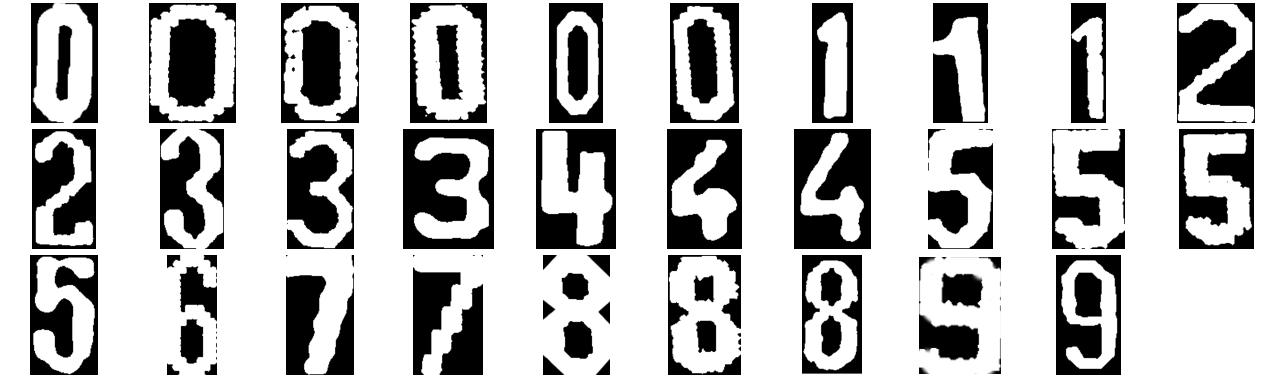
\includegraphics[width=0.95\textwidth]{img/exp_templates_used}
    \caption{Wykorzystane wzorce}
    \label{fig:used_templates}
\end{figure}

Ostatecznie niewielkim nakładem pracy można usprawnić ten etap
algorytmu poprzez dodawanie plików z~wzorcami. Przy uwzględnieniu 
konwencji nazewniczej program bez modyfikacji automatycznie
pobierze dodane pliki.

\section{Próby całego rozwiązania - podsumowanie}

Po przeprowadzeniu procedury szkolącej dla czterech detektorów
zaprojektowany został prosty algorytm wykrywania i~odczytywania numerów.
Algorytm składał się z~trzech etapów:

\begin{enumerate}
    \item Odszukanie frontu autobusu - wstępna segmentacja.
    \item Przyjmując założenie, że nadjeżdżający autobus jest autobusem
        nowego typu (z~wyświetlaczem diodowym), a~numer reprezentujący
        linię znajduje się w~lewym górnym rogu oznaczonego frontu,
        obszar poszukiwania numeru ograniczono do fragmentu lewej połowy
        frontu oraz pierwszej z~trzech części horyzontalnych. Na tym 
        fragmencie wyszukany został obszar reprezentujący numer -
        detektor kaskadowy podczas uczenia jako pozytywne próbki
        otrzymywał obrazy przedstawiające numery autobusów składające
        się od jednej do trzech cyfr.
    \item Na tak oznaczonym fragmencie uruchomiono dwa detektory
        dla których próbkami pozytywnymi były obrazy reprezentujące
        cyfry 1 oraz 8.
\end{enumerate}

Pierwszym produktem ubocznym opisanego doświadczenia był rysunek
przedstawiający rozdzielczość wykrytego numeru w~zależności
od odległości filmowanego autobusu - rysunek \ref{fig:dist2res}.

\begin{figure}[!h]
    \centering
    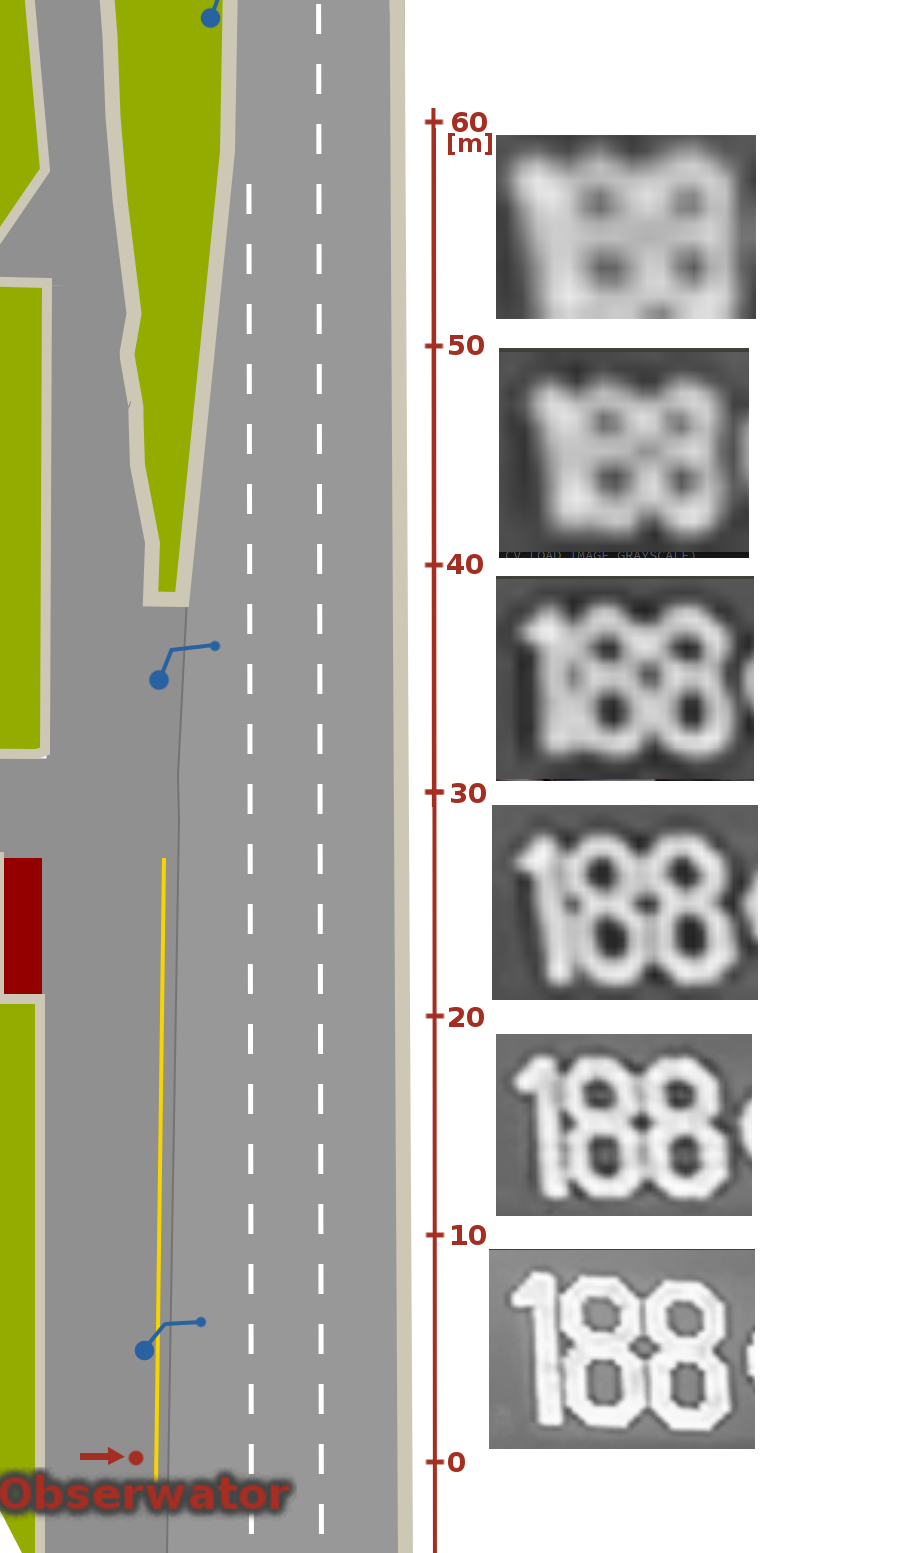
\includegraphics[height=0.9\textwidth]{img/exp_numer_od_odleglosci}
    \caption{Rozdzielczość wykrytego numeru w zależności od odległości}
    \label{fig:dist2res}
\end{figure}

Pierwszej próby dokonano dla autobusu Solaris linii 188. Odbyła się
ona na przystanku ,,Metro Politechnika 01'' w~kierunku ulicy
Marszałkowskiej.

Podczas wykonanej próby pierwsze wykrycie dla detektora
odpowiedzialnego za lokalizację frontu autobusu odnotowano około dziesięć
metrów przed pierwszym zarejestrowanym wykryciem fragmentu
przedstawiającego numer linii. Niestety z tej odległości numer był
zupełnie nieczytelny. Rozdzielczość obrazu nie pozwalała na odczytanie
numeru nawet przez człowieka.

Lokalizacja fragmentu przedstawiającego numer nastąpiła gdy autobus
znajdował się w~odległości około 50m od obserwatora. Niestety
rozdzielczość na tym etapie nie pozwalała na zastosowanie jakiejkolwiek
metody segmentacji w~celu wyodrębnienia poszczególnych cyfr. Biorąc pod
uwagę dane z~rysunku \ref{fig:dist2res} segmentacja cyfr mogła by być
zastosowana dla autobusu znajdującego się w odległości mniejszej niż
30 metrów od obserwatora. 

Ostatecznie z~zarejestrowanej sekwencji wideo wyłuskano 127 obrazów
reprezentujących front autobusu. Na trzech z~nich nie zlokalizowano
numeru. 

\subsubsection{Ostateczna architektura rozwiązania 
- dwa przebiegi testowe}

Wysokopoziomowa architektura proponowanego rozwiązania była złożona 
z~trzech etapów:
\begin{enumerate}
    \item Odnalezienie frontu autobusu - zawężenie wyszukiwania 
        do kwadratu okalającego front.
    \item Lokalizacja numeru w~obrazie reprezentującym odnaleziony
        front i~przygotowanie odseparowanego numeru jako wejścia
        do funkcji odczytującej tekst.
    \item Odczytanie numeru:
        \begin{itemize}
            \item wyszukanie potencjalnych obszarów reprezentujących
                cyfry,
            \item wyliczenie wartości reprezentującej trafność
                dopasowania cyfry w~wyznaczonym obszarze (template
                matching),
            \item wyznaczanie lokalnych maksimów oraz eliminacja 
                pozostałych teoretycznie błędnych wykryć,
            \item utworzenie ciągu znaków z~wykrytych maksimów,
                zgodnie z~kolejnością występowania w~obrazie -
                wartość odciętych lewego górnego rogu czworokąta
                okalającego.
        \end{itemize}
\end{enumerate}

\begin{figure}[!h]
    \centering
    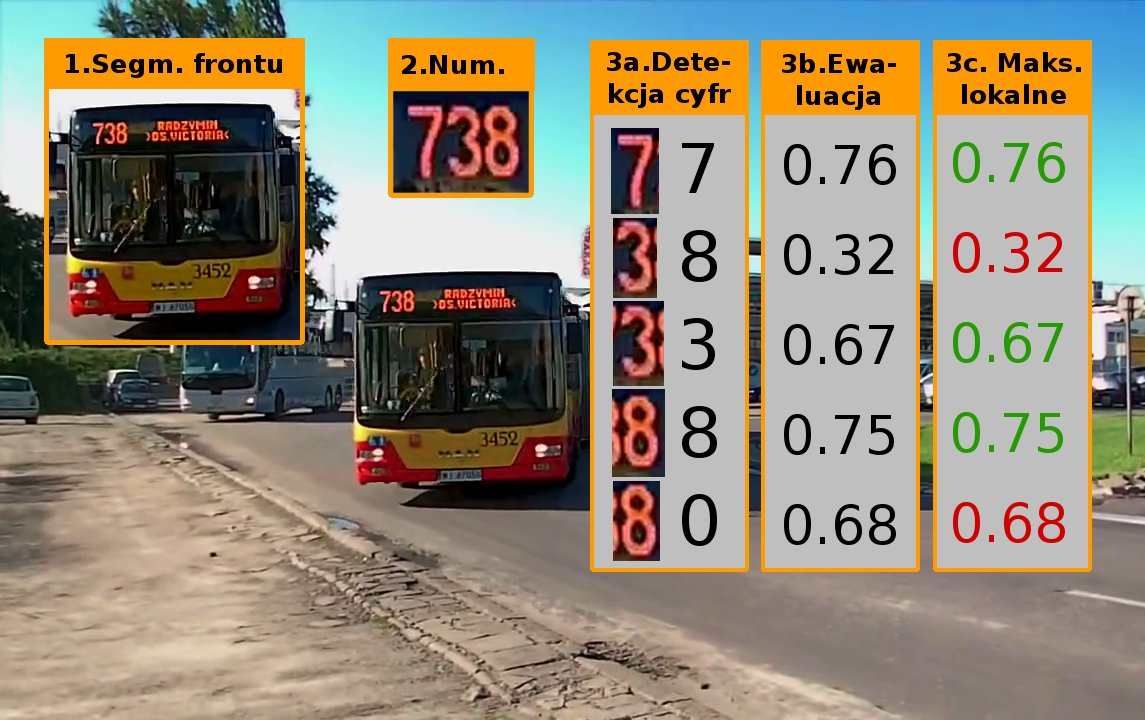
\includegraphics[width=0.9\textwidth]{img/exp_alg_explanation}
    \caption{Graficzne przedstawienie działania algorytmu na przykładzie}
    \label{fig:algexp}
\end{figure}

Rysunek \ref{fig:algexp} przedstawia przykładowy przebieg kaskady. 
Na początku wykrywany i~lokalizowany jest front autobusu.
Następnie wyłuskiwany jest fragment zawierający wyłącznie numer linii.
Ostatecznie następuje odczyt. Na zadanym fragmencie uruchamianych jest
10 detektorów dla poszczególnych cyfr. Obrazy wynikowe - potencjalnie
cyfry - przeskalowywane są do zadanej wysokości z~zachowaniem proporcji.
Dla tak przygotowanych fragmentów uruchamiana jest ewaluacja poprzez
dopasowanie wzorca lub wzorców, gdy w~zbiorze występuje kilka
reprezentacji cyfry dla różnych krojów czcionek. W~przypadku
gdy na przykład detektor trójek
wykryje ósemkę (lub na odwrót) prawdopodobnie dostanie ona niską
ocenę przy dopasowaniu tychże trójek. Ostatecznie mając
zbiór czworokątów okalających z~przypisanymi do nich wartościami
wybierane są te o~najwyższych wynikach. W~określaniu ważna jest też
odległość między cyframi. Gdyby nie wprowadzono tego kryterium
w~prezentowanym przykładzie wynik składał by się z~cyfr 7, 8 oraz 0.
Które to zero zostało wyeliminowane ze względu na zbyt bliskie położenie
względem wykrytej cyfry 8 z~wyższym wynikiem.

Tyle jeżeli chodzi o~teorię. Aby przetestować algorytm w~praktyce
popełniono pierwsza implementację testową w~języku programowania
python z~wykorzystaniem biblioteki OpenCV w wersji 2.4.9.

Jedyny test jaki wykonano był raczej potwierdzeniem, że faktycznie
rozwiązanie to może się sprawdzić. Pierwsze rezultaty uzyskane bez
dopasowywania żadnych parametrów wyglądały mniej więcej jak poniższym 
rysunku.

\begin{figure}[!h]
    \centering
    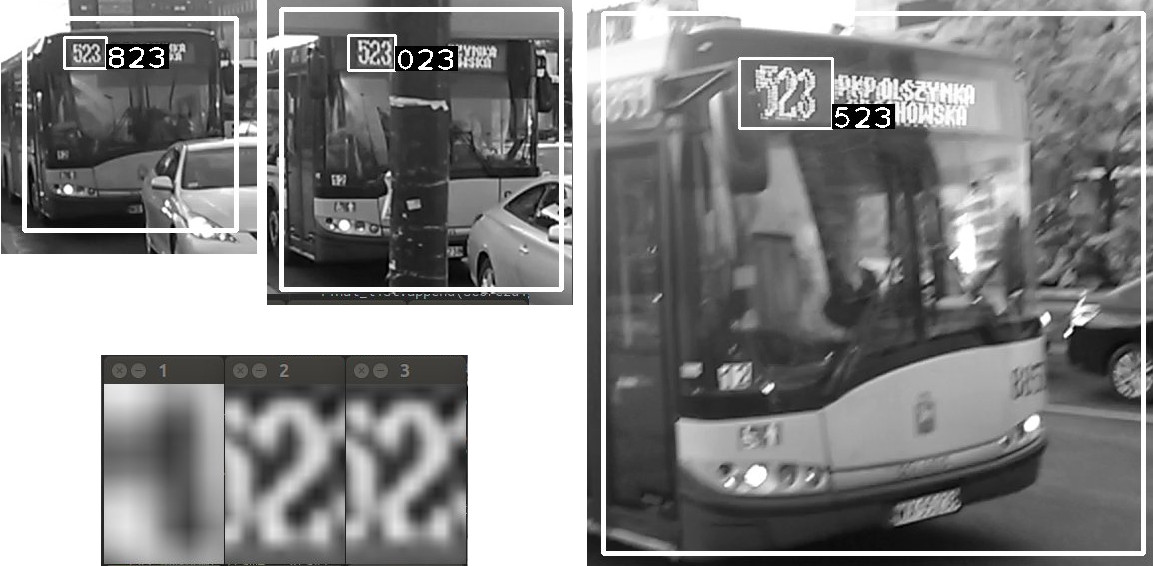
\includegraphics[width=0.9\textwidth]{img/exp_final_test}
    \caption{Ostatni test przed implementacją na telefonie}
    \label{fig:finaltest}
\end{figure}

W~lewym dolnym rogu rysunku można zaobserwować okienka prezentujące
wyniki działania detektorów do wyszukiwania cyfr. Jak nie trudno
zgadnąć były one najmniej precyzyjnym elementem całego systemu.

Jak już wspomniano był to ostatni test przed implementacją 
docelową. Jedyną zmierzoną wartością był czas potrzebny na wykrycie
frontu oraz odczytanie numeru. Na komputerze stacjonarnym z~procesorem
Intel i5 wynosił on około 100 ms na wyszukanie frontu oraz 150 ms na
odczytanie numeru. Były to wartości mocno przybliżone
tym nie mniej zapewniające wystarczający poziom pewności, że można 
będzie uruchomić to rozwiązanie na telefonie. 
